% Generated from Paper/manuscript; edit Markdown source.
\section{问题二：局部缺失下的情感预测}
\hypertarget{q2-ux95eeux9898ux5206ux6790ux4e0eux5efaux6a21ux5047ux8bbe}{%
\subsection{问题分析与建模假设}\label{q2-ux95eeux9898ux5206ux6790ux4e0eux5efaux6a21ux5047ux8bbe}}

本问利用局部缺失后的可用信息预测情感极性与强度，并分析缺失模态、位置和长度的影响。模型在编码前施加掩码，汇总有效观测并输入可用比例，以类别加权损失平衡三类识别。

采用附件2与附件3的aligned\_50版本。对齐意味着不同模态以相同序列位置组织，不能据此认定各位置具有相同持续秒数。附件2未提供逐词时间戳，因此缺失长度以有效特征位置数及比例表述，以原特征索引保留位置。

建模采用以下可检验假设。第一，字段内相同样本索引与相同对齐位置具有一致的组织含义。第二，依题意，有效区域内音视频整条特征向量为零表示不可观测，单个坐标为零仍是合法观测。第三，缺失敏感性按固定特征位置规则评价，结论适用于所构造的缺失模式。第四，监督标签遵循负值、零值、正值分别对应负向、中性、正向的定义。

尾部各模态同时为零且缺少分隔词元时，保留长度歧义标记。附件3对齐版的27条样本有131个未知词占位，对应音视位置同时全零、文本注意力为1；本文所列结果采用保留占位的固定输入口径，位置存在与词义可用状态分别记录。

\hypertarget{q2-ux6570ux636eux9884ux5904ux7406ux4e0eux7f3aux5931ux8868ux793a}{%
\subsection{数据预处理与缺失表示}\label{q2-ux6570ux636eux9884ux5904ux7406ux4e0eux7f3aux5931ux8868ux793a}}

\hypertarget{q2-ux8f93ux5165ux7ec4ux7ec7ux4e0eux89c2ux6d4bux63a9ux7801}{%
\subsubsection{输入组织与观测掩码}\label{q2-ux8f93ux5165ux7ec4ux7ec7ux4e0eux89c2ux6d4bux63a9ux7801}}

训练数据包含text\_bert、audio、vision及标签。文本统一使用text\_bert中的词元编号；训练与专项推理保持相同输入接口。已核验训练、验证与测试共4850条样本的BERT分词编号。附件3的text\_bert虽为浮点存储，读取时先验证数值有限且为整数，再转为整型编号。

\begin{equation}
X_i^a\in\mathbb{R}^{T\times74},\quad X_i^v\in\mathbb{R}^{T\times35},\quad T=50\label{q2-eq1}
\end{equation}

\begin{PaperTable}{3}

\begin{table}[!htbp]
\centering\caption{主要符号与维度\label{q2-tab2}}
\begin{tabular}{@{}lll@{}}
\toprule
\begin{minipage}[b]{\dimexpr 0.230000\linewidth-0.920000\tabcolsep\relax}\raggedright
符号\strut
\end{minipage} & \begin{minipage}[b]{\dimexpr 0.440000\linewidth-1.760000\tabcolsep\relax}\raggedright
含义\strut
\end{minipage} & \begin{minipage}[b]{\dimexpr 0.330000\linewidth-1.320000\tabcolsep\relax}\raggedright
维度或范围\strut
\end{minipage}\tabularnewline
\midrule

\begin{minipage}[t]{\dimexpr 0.230000\linewidth-0.920000\tabcolsep\relax}\raggedright
i，j，m\strut
\end{minipage} & \begin{minipage}[t]{\dimexpr 0.440000\linewidth-1.760000\tabcolsep\relax}\raggedright
样本、位置、模态索引\strut
\end{minipage} & \begin{minipage}[t]{\dimexpr 0.330000\linewidth-1.320000\tabcolsep\relax}\raggedright
m∈\{t,a,v\}\strut
\end{minipage}\tabularnewline
\begin{minipage}[t]{\dimexpr 0.230000\linewidth-0.920000\tabcolsep\relax}\raggedright
tᵢ\strut
\end{minipage} & \begin{minipage}[t]{\dimexpr 0.440000\linewidth-1.760000\tabcolsep\relax}\raggedright
文本词元编号\strut
\end{minipage} & \begin{minipage}[t]{\dimexpr 0.330000\linewidth-1.320000\tabcolsep\relax}\raggedright
50；编号0至30521\strut
\end{minipage}\tabularnewline
\begin{minipage}[t]{\dimexpr 0.230000\linewidth-0.920000\tabcolsep\relax}\raggedright
Xᵢᵃ，Xᵢᵛ\strut
\end{minipage} & \begin{minipage}[t]{\dimexpr 0.440000\linewidth-1.760000\tabcolsep\relax}\raggedright
语音与视觉输入\strut
\end{minipage} & \begin{minipage}[t]{\dimexpr 0.330000\linewidth-1.320000\tabcolsep\relax}\raggedright
50×74，50×35\strut
\end{minipage}\tabularnewline
\begin{minipage}[t]{\dimexpr 0.230000\linewidth-0.920000\tabcolsep\relax}\raggedright
vᵢⱼ\strut
\end{minipage} & \begin{minipage}[t]{\dimexpr 0.440000\linewidth-1.760000\tabcolsep\relax}\raggedright
有效位置标记\strut
\end{minipage} & \begin{minipage}[t]{\dimexpr 0.330000\linewidth-1.320000\tabcolsep\relax}\raggedright
0或1\strut
\end{minipage}\tabularnewline
\begin{minipage}[t]{\dimexpr 0.230000\linewidth-0.920000\tabcolsep\relax}\raggedright
oᵢⱼᵐ，dᵢⱼᵐ\strut
\end{minipage} & \begin{minipage}[t]{\dimexpr 0.440000\linewidth-1.760000\tabcolsep\relax}\raggedright
原观测标记与人工缺失标记\strut
\end{minipage} & \begin{minipage}[t]{\dimexpr 0.330000\linewidth-1.320000\tabcolsep\relax}\raggedright
0或1\strut
\end{minipage}\tabularnewline
\begin{minipage}[t]{\dimexpr 0.230000\linewidth-0.920000\tabcolsep\relax}\raggedright
õᵢⱼᵐ\strut
\end{minipage} & \begin{minipage}[t]{\dimexpr 0.440000\linewidth-1.760000\tabcolsep\relax}\raggedright
施加缺失后的可用标记\strut
\end{minipage} & \begin{minipage}[t]{\dimexpr 0.330000\linewidth-1.320000\tabcolsep\relax}\raggedright
0或1\strut
\end{minipage}\tabularnewline
\begin{minipage}[t]{\dimexpr 0.230000\linewidth-0.920000\tabcolsep\relax}\raggedright
cᵢ，yᵢ\strut
\end{minipage} & \begin{minipage}[t]{\dimexpr 0.440000\linewidth-1.760000\tabcolsep\relax}\raggedright
极性标签与强度标签\strut
\end{minipage} & \begin{minipage}[t]{\dimexpr 0.330000\linewidth-1.320000\tabcolsep\relax}\raggedright
\{0,1,2\}；{[}−3,3{]}\strut
\end{minipage}\tabularnewline
\begin{minipage}[t]{\dimexpr 0.230000\linewidth-0.920000\tabcolsep\relax}\raggedright
pᵢ，ŷᵢ\strut
\end{minipage} & \begin{minipage}[t]{\dimexpr 0.440000\linewidth-1.760000\tabcolsep\relax}\raggedright
三类概率与预测强度\strut
\end{minipage} & \begin{minipage}[t]{\dimexpr 0.330000\linewidth-1.320000\tabcolsep\relax}\raggedright
概率单纯形；{[}−3,3{]}\strut
\end{minipage}\tabularnewline
\begin{minipage}[t]{\dimexpr 0.230000\linewidth-0.920000\tabcolsep\relax}\raggedright
hᵢᵗ，hᵢᵃ，hᵢᵛ\strut
\end{minipage} & \begin{minipage}[t]{\dimexpr 0.440000\linewidth-1.760000\tabcolsep\relax}\raggedright
三模态投影表示\strut
\end{minipage} & \begin{minipage}[t]{\dimexpr 0.330000\linewidth-1.320000\tabcolsep\relax}\raggedright
128，64，64\strut
\end{minipage}\tabularnewline
\begin{minipage}[t]{\dimexpr 0.230000\linewidth-0.920000\tabcolsep\relax}\raggedright
aᵢ，zᵢ\strut
\end{minipage} & \begin{minipage}[t]{\dimexpr 0.440000\linewidth-1.760000\tabcolsep\relax}\raggedright
三模态可用比例与融合表示\strut
\end{minipage} & \begin{minipage}[t]{\dimexpr 0.330000\linewidth-1.320000\tabcolsep\relax}\raggedright
3，128\strut
\end{minipage}\tabularnewline
\bottomrule
\end{tabular}
\end{table}

\end{PaperTable}

有效位置通过文本注意力、词元编号及音视频非零观测的并集确定可辨识边界，排除位置0与CLS、SEP特殊词元。区域内部连续全零仍保留其位置，而不压缩序列。观测掩码则分别判断文本注意力与编号有效性、音视频有限性和整向量全零情况。两类掩码分离，使填充、特殊词元与真实缺失具有不同语义。

\begin{equation}
\widetilde{o}_{ij}^{m}=v_{ij}o_{ij}^{m}(1-d_{ij}^{m})\label{q2-eq2}
\end{equation}

式\eqref{q2-eq2}将序列结构v、原观测状态o与人工移除标记d统一为模型使用的掩码。d=1表示人工移除信息，õ=1表示该位置参与编码或汇总。原观测掩码在标准化前确定并保存，人工移除在编码前生效。保留未知词占位时，文本观测表示该位置有输入，词义是否可辨识由独立状态记录。

\hypertarget{q2-ux8badux7ec3ux96c6ux7edfux8ba1ux91cfux4e0eux8f93ux5165ux5904ux7406}{%
\subsubsection{训练集统计量与输入处理}\label{q2-ux8badux7ec3ux96c6ux7edfux8ba1ux91cfux4e0eux8f93ux5165ux5904ux7406}}

音视频每维的均值和总体标准差仅由当前拟合子集的可观测位置估计。内部三折分别计算；最终训练使用附件二完整训练集统计量，并固定用于验证、测试和附件三。

\begin{equation}
\mu_k^m={\sum_{i,j}o_{ij}^m x_{ijk}^m\over\sum_{i,j}o_{ij}^m}\label{q2-eq3}
\end{equation}

\begin{equation}
\sigma_k^m=\max\left(\sqrt{{\sum_{i,j}o_{ij}^m(x_{ijk}^m-\mu_k^m)^2\over\sum_{i,j}o_{ij}^m}},10^{-5}\right)\label{q2-eq4}
\end{equation}

\begin{equation}
\widetilde{x}_{ijk}^{m}=\widetilde{o}_{ij}^{m}\,\operatorname{clip}((x_{ijk}^{m}-\mu_k^m)/\sigma_k^m,-10,10)\label{q2-eq5}
\end{equation}

式\eqref{q2-eq3}与式\eqref{q2-eq4}的求和仅覆盖拟合子集，m取语音或视觉。标准差下界为10⁻⁵，标准化后固定裁剪至{[}−10,10{]}以限制极端数值的影响；该规则在实验前已固定，不依据验证结果改变。不可观测向量置零但另保留掩码，因此模型不会把占位零当成正常测量。

\hypertarget{q2-ux7f3aux5931ux611fux77e5ux8054ux5408ux9884ux6d4bux6a21ux578bux7684ux5efaux7acb}{%
\subsection{缺失感知联合预测模型的建立}\label{q2-ux7f3aux5931ux611fux77e5ux8054ux5408ux9884ux6d4bux6a21ux578bux7684ux5efaux7acb}}

\hypertarget{q2-ux7f16ux7801ux524dux5c4fux853dux4e0eux6587ux672cux4e0aux4e0bux6587ux8868ux793a}{%
\subsubsection{编码前屏蔽与文本上下文表示}\label{q2-ux7f16ux7801ux524dux5c4fux853dux4e0eux6587ux672cux4e0aux4e0bux6587ux8868ux793a}}

文本编码器采用bert-base-uncased通用预训练权重\cite{q2-ref1,q2-ref2}：12层、12个注意力头、768维隐状态和3072维前馈层，保留完整30522词表及前50个位置嵌入。词元、位置与segment嵌入经LayerNorm、dropout后送入Transformer。

对于缺失的普通词元，先将编号置为占位值并从注意力键中屏蔽，再进行上下文编码；CLS与可辨认的SEP保留为结构边界，CLS位置始终开启以避免全屏蔽注意力的数值问题。汇总仅使用实际观测词元，特殊词元与缺失位置不进入均值。位置与边界信息作为结构输入保留。

\begin{equation}
\operatorname{Attn}(Q,K,V)=\operatorname{softmax}(QK^{\mathsf T}/\sqrt{64}+B)V\label{q2-eq6}
\end{equation}

式\eqref{q2-eq6}给出单个注意力头的核心计算。Q、K、V为线性投影，头宽为64；B在不可用键位置取−10000，其余位置取0。实现使用残差连接、后置LayerNorm和GELU前馈变换。对于缺失位置形成的查询隐状态，不在后续池化中采用，也不允许其作为有效键传递给其他位置。

\begin{equation}
\bar h_i^t={\sum_{j=1}^T\widetilde{o}_{ij}^t H_{ij}\over\max(1,\sum_{j=1}^T\widetilde{o}_{ij}^t)}\label{q2-eq7}
\end{equation}

H为最终文本隐状态。式\eqref{q2-eq7}的分母截为至少1避免空序列除零，池化结果经768→128线性层、LayerNorm与GELU；若文本完全不可用，投影后的表示再次乘以可用性指示，使其严格为零。

\hypertarget{q2-ux97f3ux89c6ux9891ux6c47ux603bux4e0eux591aux6a21ux6001ux878dux5408}{%
\subsubsection{音视频汇总与多模态融合}\label{q2-ux97f3ux89c6ux9891ux6c47ux603bux4e0eux591aux6a21ux6001ux878dux5408}}

\begin{equation}
\bar x_i^m={\sum_{j=1}^T\widetilde{o}_{ij}^m\widetilde{x}_{ij}^m\over\max(1,\sum_{j=1}^T\widetilde{o}_{ij}^m)},\quad m\in\{a,v\}\label{q2-eq8}
\end{equation}

语音和视觉采用观测掩码均值汇总，再分别通过74→64与35→64的线性层、LayerNorm和GELU。均值编码参数量较低，保留可见片段的平均信息，省略片段内部的细粒度顺序。完全缺失的模态输出置零。

\begin{equation}
a_i^m={\sum_j\widetilde{o}_{ij}^m\over\max(1,\sum_jv_{ij})},\quad z_i=\operatorname{GELU}(W_f[h_i^t;h_i^a;h_i^v;a_i]+b_f)\label{q2-eq9}
\end{equation}

式\eqref{q2-eq9}将128维文本、64维语音、64维视觉和3维可用比例拼接成259维向量，再映射为128维融合表示，训练dropout为0.2。融合层同时接收可见内容及剩余观测量；可用比例衡量输入数量，词义完整性与预测可信程度另行判断。

\begin{equation}
p_i=\operatorname{softmax}(W_cz_i+b_c),\quad\hat c_i=\arg\max_kp_{ik},\quad\hat y_i=3\tanh(w_r^{\mathsf T}z_i+b_r)\label{q2-eq10}
\end{equation}

\begin{figure}
\centering
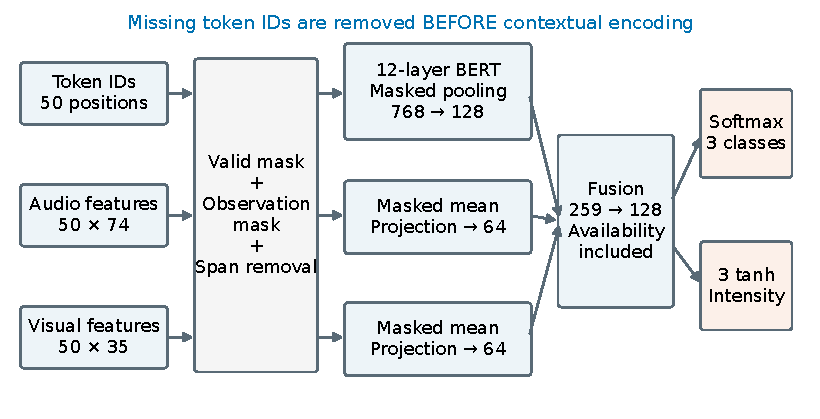
\includegraphics{../问题2/docs/paper_current/figures/r3_fig01_architecture.pdf}
\caption{模型结构与编码前缺失处理。长度50为特征位置上限，不代表50秒。融合输入包含三模态表示及可用比例。\label{q2-fig1}}
\end{figure}

分类头输出三类softmax概率，回归头通过3tanh限制强度范围。标签约定0、1、2分别为负向、中性、正向。两头共享融合表示但分别监督，因而可能出现类别与强度符号不一致；本文保存两个任务各自的输出。

\hypertarget{q2-ux7c7bux522bux5e73ux8861ux76eeux6807ux51fdux6570}{%
\subsubsection{类别平衡目标函数}\label{q2-ux7c7bux522bux5e73ux8861ux76eeux6807ux51fdux6570}}

训练集负向、中性、正向分别有967、758、1670条，最多与最少类别之比约为2.20。据此比较类别加权策略；中性类错误还可能与语义边界、表示能力及优化过程有关。

以类别频率调整经验风险\cite{q2-ref6,q2-ref7}，比较不加权、平方根逆频率与逆频率三个强度。设当前拟合子集含N条样本、第c类数量为n\_c，C=3，各内部折独立计数。

\begin{equation}
u_c=(N/(C n_c))^\alpha,\quad w_c=u_c/(C^{-1}\sum_{k=0}^{C-1}u_k),\quad\alpha\in\{0,0.5,1\}\label{q2-eq11}
\end{equation}

α=0、0.5、1分别对应不加权、平方根逆频率和逆频率。最终采用α=1，权重从第1轮开始作用。公共缩放在加权交叉熵的分子分母中相互抵消，因此将类别权重的算术均值规范为1不改变目标；若当前拟合子集缺少某类，程序明确报错而不生成无穷权重。

\begin{equation}
\mathcal L_B=-\frac{\sum_{i\in B}w_{c_i}\log p_{i,c_i}}{\sum_{i\in B}w_{c_i}}+\frac{1}{|B|}\sum_{i\in B}H_1(\hat y_i-y_i)\label{q2-eq12}
\end{equation}

\begin{equation}
H_1(e)=\begin{cases}e^2/2,&|e|\le1,\\|e|-1/2,&|e|>1.\end{cases}\label{q2-eq13}
\end{equation}

c\_i始终表示离散类别，y\_i始终表示连续强度，B表示有效批量；分类概率p的第二下标选择真实类别。加权交叉熵强调较少类别的分类误差，Huber阈值固定为1，对较大回归残差采用线性增长。两任务系数为1:1。类别权重不增加推理参数，也不将softmax概率自动校准为正确率。

\hypertarget{q2-ux8fdeux7eedux7f3aux5931ux8badux7ec3}{%
\subsubsection{连续缺失训练}\label{q2-ux8fdeux7eedux7f3aux5931ux8badux7ec3}}

\begin{equation}
k_i=\min(n_i,\max(1,\lfloor r n_i+0.5\rfloor)),\quad n_i=\sum_jv_{ij}\label{q2-eq14}
\end{equation}

对每个训练样本，以0.7概率选取一个模态施加连续缺失，模态均匀抽样，比例r从0.1、0.3、0.5中均匀抽样。式\eqref{q2-eq14}适用于有效长度nᵢ\textgreater0；空序列不额外移除位置。连续性按有效位置的顺序定义，随机起点保证所选片段在边界内。增强将人工缺失条件下的监督风险纳入训练，其效果通过消融实验评价。

\hypertarget{q2-ux6a21ux578bux6c42ux89e3ux4e0eux5b9eux9a8cux8bbeux8ba1}{%
\subsection{模型求解与实验设计}\label{q2-ux6a21ux578bux6c42ux89e3ux4e0eux5b9eux9a8cux8bbeux8ba1}}

\begin{PaperTable}{2}

\begin{table}[!htbp]
\centering\caption{固定训练参数\label{q2-tab3}}
\begin{tabular}{@{}ll@{}}
\toprule
\begin{minipage}[b]{\dimexpr 0.080000\linewidth-0.160000\tabcolsep\relax}\raggedleft
步骤\strut
\end{minipage} & \begin{minipage}[b]{\dimexpr 0.920000\linewidth-1.840000\tabcolsep\relax}\raggedright
操作\strut
\end{minipage}\tabularnewline
\midrule

\begin{minipage}[t]{\dimexpr 0.080000\linewidth-0.160000\tabcolsep\relax}\raggedleft
1\strut
\end{minipage} & \begin{minipage}[t]{\dimexpr 0.920000\linewidth-1.840000\tabcolsep\relax}\raggedright
保留附件二给定的数据划分；在训练集内按原视频标识生成三折，各折视频组不重叠。\strut
\end{minipage}\tabularnewline
\begin{minipage}[t]{\dimexpr 0.080000\linewidth-0.160000\tabcolsep\relax}\raggedleft
2\strut
\end{minipage} & \begin{minipage}[t]{\dimexpr 0.920000\linewidth-1.840000\tabcolsep\relax}\raggedright
各折只以拟合样本估计标准化参数和类别频率；按阶段协议固定预训练词表。\strut
\end{minipage}\tabularnewline
\begin{minipage}[t]{\dimexpr 0.080000\linewidth-0.160000\tabcolsep\relax}\raggedleft
3\strut
\end{minipage} & \begin{minipage}[t]{\dimexpr 0.920000\linewidth-1.840000\tabcolsep\relax}\raggedright
初始化预训练编码器和预测头；每个批量在编码前按规则生成局部缺失掩码。\strut
\end{minipage}\tabularnewline
\begin{minipage}[t]{\dimexpr 0.080000\linewidth-0.160000\tabcolsep\relax}\raggedleft
4\strut
\end{minipage} & \begin{minipage}[t]{\dimexpr 0.920000\linewidth-1.840000\tabcolsep\relax}\raggedright
计算加权交叉熵与Huber损失，按有效批量累积梯度，裁剪后以AdamW更新。\strut
\end{minipage}\tabularnewline
\begin{minipage}[t]{\dimexpr 0.080000\linewidth-0.160000\tabcolsep\relax}\raggedleft
5\strut
\end{minipage} & \begin{minipage}[t]{\dimexpr 0.920000\linewidth-1.840000\tabcolsep\relax}\raggedright
内部每轮评价完整输入和九类固定缺失场景；按预定分数保存最佳轮次并早停。\strut
\end{minipage}\tabularnewline
\begin{minipage}[t]{\dimexpr 0.080000\linewidth-0.160000\tabcolsep\relax}\raggedleft
6\strut
\end{minipage} & \begin{minipage}[t]{\dimexpr 0.920000\linewidth-1.840000\tabcolsep\relax}\raggedright
对完成三折且满足保护条件的候选排序；以最佳轮数中位数固定正式训练轮数。\strut
\end{minipage}\tabularnewline
\begin{minipage}[t]{\dimexpr 0.080000\linewidth-0.160000\tabcolsep\relax}\raggedleft
7\strut
\end{minipage} & \begin{minipage}[t]{\dimexpr 0.920000\linewidth-1.840000\tabcolsep\relax}\raggedright
在附件二训练集上用三个随机种子分别重新训练，并在验证集上评价；固定模型后报告测试集结果，其解释范围见共用数据约定。\strut
\end{minipage}\tabularnewline
\bottomrule
\end{tabular}
\end{table}

\end{PaperTable}

\begin{PaperTable}{2}

\begin{table}[!htbp]
\centering\caption{模型求解与实验设计}
\begin{tabular}{@{}ll@{}}
\toprule
\begin{minipage}[b]{\dimexpr 0.310000\linewidth-0.620000\tabcolsep\relax}\raggedright
项目\strut
\end{minipage} & \begin{minipage}[b]{\dimexpr 0.690000\linewidth-1.380000\tabcolsep\relax}\raggedright
取值\strut
\end{minipage}\tabularnewline
\midrule

\begin{minipage}[t]{\dimexpr 0.310000\linewidth-0.620000\tabcolsep\relax}\raggedright
编码器学习率\strut
\end{minipage} & \begin{minipage}[t]{\dimexpr 0.690000\linewidth-1.380000\tabcolsep\relax}\raggedright
2×10⁻⁵\strut
\end{minipage}\tabularnewline
\begin{minipage}[t]{\dimexpr 0.310000\linewidth-0.620000\tabcolsep\relax}\raggedright
投影与预测头学习率\strut
\end{minipage} & \begin{minipage}[t]{\dimexpr 0.690000\linewidth-1.380000\tabcolsep\relax}\raggedright
5×10⁻⁴\strut
\end{minipage}\tabularnewline
\begin{minipage}[t]{\dimexpr 0.310000\linewidth-0.620000\tabcolsep\relax}\raggedright
优化器与权重衰减\strut
\end{minipage} & \begin{minipage}[t]{\dimexpr 0.690000\linewidth-1.380000\tabcolsep\relax}\raggedright
AdamW；0.01；偏置和归一化参数不衰减\strut
\end{minipage}\tabularnewline
\begin{minipage}[t]{\dimexpr 0.310000\linewidth-0.620000\tabcolsep\relax}\raggedright
有效批量与梯度裁剪\strut
\end{minipage} & \begin{minipage}[t]{\dimexpr 0.690000\linewidth-1.380000\tabcolsep\relax}\raggedright
32；梯度范数上限1\strut
\end{minipage}\tabularnewline
\begin{minipage}[t]{\dimexpr 0.310000\linewidth-0.620000\tabcolsep\relax}\raggedright
学习率计划\strut
\end{minipage} & \begin{minipage}[t]{\dimexpr 0.690000\linewidth-1.380000\tabcolsep\relax}\raggedright
前10\%更新线性预热，其后线性衰减\strut
\end{minipage}\tabularnewline
\begin{minipage}[t]{\dimexpr 0.310000\linewidth-0.620000\tabcolsep\relax}\raggedright
内部训练预算\strut
\end{minipage} & \begin{minipage}[t]{\dimexpr 0.690000\linewidth-1.380000\tabcolsep\relax}\raggedright
12层模型最多6轮；连续3轮无改善早停\strut
\end{minipage}\tabularnewline
\begin{minipage}[t]{\dimexpr 0.310000\linewidth-0.620000\tabcolsep\relax}\raggedright
训练与推理精度\strut
\end{minipage} & \begin{minipage}[t]{\dimexpr 0.690000\linewidth-1.380000\tabcolsep\relax}\raggedright
CUDA BF16自动混合精度训练；FP32评价；关闭TF32\strut
\end{minipage}\tabularnewline
\begin{minipage}[t]{\dimexpr 0.310000\linewidth-0.620000\tabcolsep\relax}\raggedright
随机种子\strut
\end{minipage} & \begin{minipage}[t]{\dimexpr 0.690000\linewidth-1.380000\tabcolsep\relax}\raggedright
三折分组240924；重复实验42、2026、3407\strut
\end{minipage}\tabularnewline
\begin{minipage}[t]{\dimexpr 0.310000\linewidth-0.620000\tabcolsep\relax}\raggedright
连续缺失增强\strut
\end{minipage} & \begin{minipage}[t]{\dimexpr 0.690000\linewidth-1.380000\tabcolsep\relax}\raggedright
概率0.7；三模态与三个比例均匀抽样\strut
\end{minipage}\tabularnewline
\begin{minipage}[t]{\dimexpr 0.310000\linewidth-0.620000\tabcolsep\relax}\raggedright
损失权重\strut
\end{minipage} & \begin{minipage}[t]{\dimexpr 0.690000\linewidth-1.380000\tabcolsep\relax}\raggedright
加权交叉熵:Huber=1:1\strut
\end{minipage}\tabularnewline
\bottomrule
\end{tabular}
\end{table}

\end{PaperTable}

AdamW采用解耦权重衰减\cite{q2-ref3}。有效批量固定为32；显存不足时允许微批量缩至16或8并累计贡献，不能对类别组成不同的微批量加权均值简单平均。对批量\(B\)的互不相交分块\(B_j\)，分类分母使用完整\(B\)的权重和，回归分母使用\(|B|\)。固定训练轮数后，仅在训练结束时评价验证集，不根据逐轮验证结果选择检查点。

\begin{equation}
\mathcal L_B=\sum_j\left[-\frac{\sum_{i\in B_j}w_{c_i}\log p_{i,c_i}}{\sum_{i\in B}w_{c_i}}+\frac{\sum_{i\in B_j}H_1(\hat y_i-y_i)}{|B|}\right]\label{q2-eq15}
\end{equation}

\begin{equation}
\operatorname{MAE}={1\over N}\sum_i|\hat y_i-y_i|,\quad S={1\over2}\overline{F1}_{miss}+{1\over2}(1-\overline{MAE}_{miss}/6)\label{q2-eq17}
\end{equation}

除式\eqref{q2-eq17}的选择分数外，按共用评价约定报告Accuracy、Macro-F1、各类别F1、MAE与Pearson。F1对三类等权求平均，分母为零的类别按0计；Pearson在样本不足或真值、预测恒定时记为未定义。综合分数S是本文预先设定的模型选择准则，不代表赛题评分规则。

验证主场景为文本、语音、视觉分别缺失10\%、30\%、50\%，共9类；每个样本的随机起点由固定种子、样本ID和场景名称的SHA256确定。补充场景采用前部、中部、后部以及分成最多三段的多个短区间，共36类。多个短片段不保证彼此间隔非零，极短样本中可能合并，报告按实际移除位置统计而非假定严格分离。

同组对照共享评价场景；固定4轮增强实验还分离样本顺序与增强随机数，保持配对训练的样本顺序一致。S使用九个场景各自指标的算术平均。完整输入clean表示没有额外人工缺失，仍可能包含原始自然缺失。人工选择的位置若原本不可观测，不会产生额外的信息移除；因此同时记录所选位置数和新增不可观测位置数。

类别权重候选须至少在两个内部折提高S，且完整输入三折平均Macro-F1下降不超过0.01、MAE增加不超过0.03；取合格者中平均S最高者，与基线采用相同的三个随机种子进行配对实验。正式训练固定为内部最佳轮数中位数4轮，部署使用种子42。

附件二验证集用于比较选定方案的性能并分析缺失规律；历史测试观察及评价范围按共用数据约定说明。

\hypertarget{q2-ux7ed3ux679cux68c0ux9a8cux4e0eux6a21ux578bux6bd4ux8f83}{%
\subsection{结果检验与模型比较}\label{q2-ux7ed3ux679cux68c0ux9a8cux4e0eux6a21ux578bux6bd4ux8f83}}

最终模型采用种子42、固定4轮的重训权重，缺失规律、错误分析和附件三预测均使用此版本。以下先给出训练方案选择依据，再报告最终性能。视频分组配对Bootstrap反映固定模型的样本抽样不确定性，三种子实验反映训练波动。

\hypertarget{q2-ux9884ux8badux7ec3ux65b9ux6848ux4e0eux7f3aux5931ux589eux5f3aux5bf9ux7167}{%
\subsubsection{预训练方案与缺失增强对照}\label{q2-ux9884ux8badux7ec3ux65b9ux6848ux4e0eux7f3aux5931ux589eux5f3aux5bf9ux7167}}

\begin{PaperTable}{6}

\begin{table}[!htbp]
\centering\caption{内部三折平均结果\label{q2-tab4}}
\begin{tabular}{@{}llllll@{}}
\toprule
\begin{minipage}[b]{\dimexpr 0.350000\linewidth-3.500000\tabcolsep\relax}\raggedright
模型\strut
\end{minipage} & \begin{minipage}[b]{\dimexpr 0.130000\linewidth-1.300000\tabcolsep\relax}\raggedleft
完整F1\strut
\end{minipage} & \begin{minipage}[b]{\dimexpr 0.140000\linewidth-1.400000\tabcolsep\relax}\raggedleft
完整MAE\strut
\end{minipage} & \begin{minipage}[b]{\dimexpr 0.130000\linewidth-1.300000\tabcolsep\relax}\raggedleft
缺失F1\strut
\end{minipage} & \begin{minipage}[b]{\dimexpr 0.140000\linewidth-1.400000\tabcolsep\relax}\raggedleft
缺失MAE\strut
\end{minipage} & \begin{minipage}[b]{\dimexpr 0.110000\linewidth-1.100000\tabcolsep\relax}\raggedleft
S\strut
\end{minipage}\tabularnewline
\midrule

\begin{minipage}[t]{\dimexpr 0.350000\linewidth-3.500000\tabcolsep\relax}\raggedright
两层蒸馏基线\strut
\end{minipage} & \begin{minipage}[t]{\dimexpr 0.130000\linewidth-1.300000\tabcolsep\relax}\raggedleft
0.5575\strut
\end{minipage} & \begin{minipage}[t]{\dimexpr 0.140000\linewidth-1.400000\tabcolsep\relax}\raggedleft
0.6938\strut
\end{minipage} & \begin{minipage}[t]{\dimexpr 0.130000\linewidth-1.300000\tabcolsep\relax}\raggedleft
0.5475\strut
\end{minipage} & \begin{minipage}[t]{\dimexpr 0.140000\linewidth-1.400000\tabcolsep\relax}\raggedleft
0.7073\strut
\end{minipage} & \begin{minipage}[t]{\dimexpr 0.110000\linewidth-1.100000\tabcolsep\relax}\raggedleft
0.7148\strut
\end{minipage}\tabularnewline
\begin{minipage}[t]{\dimexpr 0.350000\linewidth-3.500000\tabcolsep\relax}\raggedright
12层裁剪词表＋缺失训练\strut
\end{minipage} & \begin{minipage}[t]{\dimexpr 0.130000\linewidth-1.300000\tabcolsep\relax}\raggedleft
0.6025\strut
\end{minipage} & \begin{minipage}[t]{\dimexpr 0.140000\linewidth-1.400000\tabcolsep\relax}\raggedleft
0.6094\strut
\end{minipage} & \begin{minipage}[t]{\dimexpr 0.130000\linewidth-1.300000\tabcolsep\relax}\raggedleft
0.5857\strut
\end{minipage} & \begin{minipage}[t]{\dimexpr 0.140000\linewidth-1.400000\tabcolsep\relax}\raggedleft
0.6301\strut
\end{minipage} & \begin{minipage}[t]{\dimexpr 0.110000\linewidth-1.100000\tabcolsep\relax}\raggedleft
0.7403\strut
\end{minipage}\tabularnewline
\begin{minipage}[t]{\dimexpr 0.350000\linewidth-3.500000\tabcolsep\relax}\raggedright
12层完整词表＋缺失训练\strut
\end{minipage} & \begin{minipage}[t]{\dimexpr 0.130000\linewidth-1.300000\tabcolsep\relax}\raggedleft
0.6218\strut
\end{minipage} & \begin{minipage}[t]{\dimexpr 0.140000\linewidth-1.400000\tabcolsep\relax}\raggedleft
0.6050\strut
\end{minipage} & \begin{minipage}[t]{\dimexpr 0.130000\linewidth-1.300000\tabcolsep\relax}\raggedleft
0.6038\strut
\end{minipage} & \begin{minipage}[t]{\dimexpr 0.140000\linewidth-1.400000\tabcolsep\relax}\raggedleft
0.6241\strut
\end{minipage} & \begin{minipage}[t]{\dimexpr 0.110000\linewidth-1.100000\tabcolsep\relax}\raggedleft
0.7499\strut
\end{minipage}\tabularnewline
\begin{minipage}[t]{\dimexpr 0.350000\linewidth-3.500000\tabcolsep\relax}\raggedright
12层完整词表 无缺失增强\strut
\end{minipage} & \begin{minipage}[t]{\dimexpr 0.130000\linewidth-1.300000\tabcolsep\relax}\raggedleft
0.6231\strut
\end{minipage} & \begin{minipage}[t]{\dimexpr 0.140000\linewidth-1.400000\tabcolsep\relax}\raggedleft
0.6031\strut
\end{minipage} & \begin{minipage}[t]{\dimexpr 0.130000\linewidth-1.300000\tabcolsep\relax}\raggedleft
0.6044\strut
\end{minipage} & \begin{minipage}[t]{\dimexpr 0.140000\linewidth-1.400000\tabcolsep\relax}\raggedleft
0.6227\strut
\end{minipage} & \begin{minipage}[t]{\dimexpr 0.110000\linewidth-1.100000\tabcolsep\relax}\raggedleft
0.7503\strut
\end{minipage}\tabularnewline
\bottomrule
\end{tabular}
\end{table}

\end{PaperTable}

表\ref{q2-tab4}中F1为Macro-F1，数值为视频分组内部三折的算术均值。完整词表方案与关闭缺失增强方案采用相同训练协议。关闭增强后S增加0.0004、缺失F1增加0.0006、缺失MAE降低0.0015。该对照使用未加权分类损失，两组按各自内部验证分数选择轮次，因此评价的是包含早停的训练策略。

完整词表相对于裁剪词表12层模型，三折平均S变化为+0.0096，完整F1变化为+0.0193，完整MAE变化为-0.0044。该比较提供词表保留策略的经验依据；由于词表维度变化也会影响同种子下后续随机初始化序列，且开发阶段只使用一个训练种子，不能将差异完全归因为未见词元本身。

未加权、带早停的增强对照与最终加权、固定4轮训练方案不同。后文补充仅改变增强方式的配对实验，用于直接检验最终训练方案中连续缺失训练的作用。

保留的两层实验分别检验文本单模态、多模态输入、连续缺失增强、蒸馏与随机初始化；四层实验检验另一种编码深度。蒸馏模型与四层模型的内部S差距很小，不能仅凭排序宣称其具有显著优势。两层与12层模型训练轮数及训练目标可能不同，跨结构的差异包含多个因素的共同影响。

\hypertarget{q2-ux7c7bux522bux6743ux91cdux7684ux5185ux90e8ux914dux5bf9ux6bd4ux8f83}{%
\subsubsection{类别权重的内部配对比较}\label{q2-ux7c7bux522bux6743ux91cdux7684ux5185ux90e8ux914dux5bf9ux6bd4ux8f83}}

内部开发继续使用不加权基线按视频分组的三折。每个候选仅改变分类权重强度，随机种子42，最多6轮、早停耐心3轮；标准化、原始预训练权重、完整词表、连续缺失训练概率0.7和AdamW参数保持一致。以九类主要缺失场景上的既有综合分数S选择最佳轮次，再用最佳轮数中位数确定在附件二完整训练集上重新训练的固定轮数。

在相同环境与训练方案下复算不加权配置第1折，217个参数张量逐项一致，最大绝对差和选择分数差均为0.0，据此复用该组对照。逐位一致性仅在上述环境中验证。

\begin{PaperTable}{6}

\begin{table}[!htbp]
\centering\caption{内部三折算术均值\label{q2-tab5}}
\begin{tabular}{@{}llllll@{}}
\toprule
\begin{minipage}[b]{\dimexpr 0.240000\linewidth-2.400000\tabcolsep\relax}\raggedright
配置\strut
\end{minipage} & \begin{minipage}[b]{\dimexpr 0.150000\linewidth-1.500000\tabcolsep\relax}\raggedleft
完整F1\strut
\end{minipage} & \begin{minipage}[b]{\dimexpr 0.160000\linewidth-1.600000\tabcolsep\relax}\raggedleft
完整MAE\strut
\end{minipage} & \begin{minipage}[b]{\dimexpr 0.150000\linewidth-1.500000\tabcolsep\relax}\raggedleft
缺失F1\strut
\end{minipage} & \begin{minipage}[b]{\dimexpr 0.160000\linewidth-1.600000\tabcolsep\relax}\raggedleft
缺失MAE\strut
\end{minipage} & \begin{minipage}[b]{\dimexpr 0.140000\linewidth-1.400000\tabcolsep\relax}\raggedleft
S\strut
\end{minipage}\tabularnewline
\midrule

\begin{minipage}[t]{\dimexpr 0.240000\linewidth-2.400000\tabcolsep\relax}\raggedright
不加权参照\strut
\end{minipage} & \begin{minipage}[t]{\dimexpr 0.150000\linewidth-1.500000\tabcolsep\relax}\raggedleft
0.6218\strut
\end{minipage} & \begin{minipage}[t]{\dimexpr 0.160000\linewidth-1.600000\tabcolsep\relax}\raggedleft
0.6050\strut
\end{minipage} & \begin{minipage}[t]{\dimexpr 0.150000\linewidth-1.500000\tabcolsep\relax}\raggedleft
0.6038\strut
\end{minipage} & \begin{minipage}[t]{\dimexpr 0.160000\linewidth-1.600000\tabcolsep\relax}\raggedleft
0.6241\strut
\end{minipage} & \begin{minipage}[t]{\dimexpr 0.140000\linewidth-1.400000\tabcolsep\relax}\raggedleft
0.7499\strut
\end{minipage}\tabularnewline
\begin{minipage}[t]{\dimexpr 0.240000\linewidth-2.400000\tabcolsep\relax}\raggedright
平方根权重\strut
\end{minipage} & \begin{minipage}[t]{\dimexpr 0.150000\linewidth-1.500000\tabcolsep\relax}\raggedleft
0.6294\strut
\end{minipage} & \begin{minipage}[t]{\dimexpr 0.160000\linewidth-1.600000\tabcolsep\relax}\raggedleft
0.6059\strut
\end{minipage} & \begin{minipage}[t]{\dimexpr 0.150000\linewidth-1.500000\tabcolsep\relax}\raggedleft
0.6092\strut
\end{minipage} & \begin{minipage}[t]{\dimexpr 0.160000\linewidth-1.600000\tabcolsep\relax}\raggedleft
0.6250\strut
\end{minipage} & \begin{minipage}[t]{\dimexpr 0.140000\linewidth-1.400000\tabcolsep\relax}\raggedleft
0.7525\strut
\end{minipage}\tabularnewline
\begin{minipage}[t]{\dimexpr 0.240000\linewidth-2.400000\tabcolsep\relax}\raggedright
逆频率权重\strut
\end{minipage} & \begin{minipage}[t]{\dimexpr 0.150000\linewidth-1.500000\tabcolsep\relax}\raggedleft
0.6327\strut
\end{minipage} & \begin{minipage}[t]{\dimexpr 0.160000\linewidth-1.600000\tabcolsep\relax}\raggedleft
0.6147\strut
\end{minipage} & \begin{minipage}[t]{\dimexpr 0.150000\linewidth-1.500000\tabcolsep\relax}\raggedleft
0.6124\strut
\end{minipage} & \begin{minipage}[t]{\dimexpr 0.160000\linewidth-1.600000\tabcolsep\relax}\raggedleft
0.6325\strut
\end{minipage} & \begin{minipage}[t]{\dimexpr 0.140000\linewidth-1.400000\tabcolsep\relax}\raggedleft
0.7535\strut
\end{minipage}\tabularnewline
\bottomrule
\end{tabular}
\end{table}

\end{PaperTable}

平方根权重和逆频率权重均在2/3折提高S并满足保护条件，平均增量分别为0.00263和0.00360，中性F1均值分别为0.4611和0.4646。据平均S选取逆频率权重。各配置采用内部验证选定的最佳轮次，因此结果评价同一预算下的训练方案，包含模型选择的影响。

\hypertarget{q2-ux8badux7ec3ux65b9ux6848ux9009ux62e9ux4e2dux7684ux91cdux590dux5b9eux9a8cux4e0eux6027ux80fdux53d6ux820d}{%
\subsubsection{训练方案选择中的重复实验与性能取舍}\label{q2-ux8badux7ec3ux65b9ux6848ux9009ux62e9ux4e2dux7684ux91cdux590dux5b9eux9a8cux4e0eux6027ux80fdux53d6ux820d}}

\begin{PaperTable}{4}

\begin{table}[!htbp]
\centering\caption{验证集上三个随机种子实验结果的均值与样本标准差\label{q2-tab7}}
\begin{tabular}{@{}llll@{}}
\toprule
\begin{minipage}[b]{\dimexpr 0.290000\linewidth-1.740000\tabcolsep\relax}\raggedright
指标\strut
\end{minipage} & \begin{minipage}[b]{\dimexpr 0.280000\linewidth-1.680000\tabcolsep\relax}\raggedleft
不加权基线参照\strut
\end{minipage} & \begin{minipage}[b]{\dimexpr 0.280000\linewidth-1.680000\tabcolsep\relax}\raggedleft
类别平衡模型\strut
\end{minipage} & \begin{minipage}[b]{\dimexpr 0.150000\linewidth-0.900000\tabcolsep\relax}\raggedleft
均值差\strut
\end{minipage}\tabularnewline
\midrule

\begin{minipage}[t]{\dimexpr 0.290000\linewidth-1.740000\tabcolsep\relax}\raggedright
完整Accuracy\strut
\end{minipage} & \begin{minipage}[t]{\dimexpr 0.280000\linewidth-1.680000\tabcolsep\relax}\raggedleft
0.6369 ± 0.0042\strut
\end{minipage} & \begin{minipage}[t]{\dimexpr 0.280000\linewidth-1.680000\tabcolsep\relax}\raggedleft
0.6277 ± 0.0060\strut
\end{minipage} & \begin{minipage}[t]{\dimexpr 0.150000\linewidth-0.900000\tabcolsep\relax}\raggedleft
-0.0092\strut
\end{minipage}\tabularnewline
\begin{minipage}[t]{\dimexpr 0.290000\linewidth-1.740000\tabcolsep\relax}\raggedright
完整Macro-F1\strut
\end{minipage} & \begin{minipage}[t]{\dimexpr 0.280000\linewidth-1.680000\tabcolsep\relax}\raggedleft
0.5959 ± 0.0059\strut
\end{minipage} & \begin{minipage}[t]{\dimexpr 0.280000\linewidth-1.680000\tabcolsep\relax}\raggedleft
0.6163 ± 0.0040\strut
\end{minipage} & \begin{minipage}[t]{\dimexpr 0.150000\linewidth-0.900000\tabcolsep\relax}\raggedleft
+0.0204\strut
\end{minipage}\tabularnewline
\begin{minipage}[t]{\dimexpr 0.290000\linewidth-1.740000\tabcolsep\relax}\raggedright
完整MAE\strut
\end{minipage} & \begin{minipage}[t]{\dimexpr 0.280000\linewidth-1.680000\tabcolsep\relax}\raggedleft
0.5783 ± 0.0060\strut
\end{minipage} & \begin{minipage}[t]{\dimexpr 0.280000\linewidth-1.680000\tabcolsep\relax}\raggedleft
0.5790 ± 0.0099\strut
\end{minipage} & \begin{minipage}[t]{\dimexpr 0.150000\linewidth-0.900000\tabcolsep\relax}\raggedleft
+0.0006\strut
\end{minipage}\tabularnewline
\begin{minipage}[t]{\dimexpr 0.290000\linewidth-1.740000\tabcolsep\relax}\raggedright
完整Pearson\strut
\end{minipage} & \begin{minipage}[t]{\dimexpr 0.280000\linewidth-1.680000\tabcolsep\relax}\raggedleft
0.6815 ± 0.0063\strut
\end{minipage} & \begin{minipage}[t]{\dimexpr 0.280000\linewidth-1.680000\tabcolsep\relax}\raggedleft
0.6816 ± 0.0086\strut
\end{minipage} & \begin{minipage}[t]{\dimexpr 0.150000\linewidth-0.900000\tabcolsep\relax}\raggedleft
+0.0001\strut
\end{minipage}\tabularnewline
\begin{minipage}[t]{\dimexpr 0.290000\linewidth-1.740000\tabcolsep\relax}\raggedright
负向类别F1\strut
\end{minipage} & \begin{minipage}[t]{\dimexpr 0.280000\linewidth-1.680000\tabcolsep\relax}\raggedleft
0.6770 ± 0.0109\strut
\end{minipage} & \begin{minipage}[t]{\dimexpr 0.280000\linewidth-1.680000\tabcolsep\relax}\raggedleft
0.6728 ± 0.0070\strut
\end{minipage} & \begin{minipage}[t]{\dimexpr 0.150000\linewidth-0.900000\tabcolsep\relax}\raggedleft
-0.0042\strut
\end{minipage}\tabularnewline
\begin{minipage}[t]{\dimexpr 0.290000\linewidth-1.740000\tabcolsep\relax}\raggedright
中性类别F1\strut
\end{minipage} & \begin{minipage}[t]{\dimexpr 0.280000\linewidth-1.680000\tabcolsep\relax}\raggedleft
0.3871 ± 0.0133\strut
\end{minipage} & \begin{minipage}[t]{\dimexpr 0.280000\linewidth-1.680000\tabcolsep\relax}\raggedleft
0.4808 ± 0.0062\strut
\end{minipage} & \begin{minipage}[t]{\dimexpr 0.150000\linewidth-0.900000\tabcolsep\relax}\raggedleft
+0.0937\strut
\end{minipage}\tabularnewline
\begin{minipage}[t]{\dimexpr 0.290000\linewidth-1.740000\tabcolsep\relax}\raggedright
正向类别F1\strut
\end{minipage} & \begin{minipage}[t]{\dimexpr 0.280000\linewidth-1.680000\tabcolsep\relax}\raggedleft
0.7238 ± 0.0020\strut
\end{minipage} & \begin{minipage}[t]{\dimexpr 0.280000\linewidth-1.680000\tabcolsep\relax}\raggedleft
0.6954 ± 0.0140\strut
\end{minipage} & \begin{minipage}[t]{\dimexpr 0.150000\linewidth-0.900000\tabcolsep\relax}\raggedleft
-0.0284\strut
\end{minipage}\tabularnewline
\begin{minipage}[t]{\dimexpr 0.290000\linewidth-1.740000\tabcolsep\relax}\raggedright
缺失平均Macro-F1\strut
\end{minipage} & \begin{minipage}[t]{\dimexpr 0.280000\linewidth-1.680000\tabcolsep\relax}\raggedleft
0.5862 ± 0.0018\strut
\end{minipage} & \begin{minipage}[t]{\dimexpr 0.280000\linewidth-1.680000\tabcolsep\relax}\raggedleft
0.6026 ± 0.0013\strut
\end{minipage} & \begin{minipage}[t]{\dimexpr 0.150000\linewidth-0.900000\tabcolsep\relax}\raggedleft
+0.0164\strut
\end{minipage}\tabularnewline
\begin{minipage}[t]{\dimexpr 0.290000\linewidth-1.740000\tabcolsep\relax}\raggedright
缺失平均MAE\strut
\end{minipage} & \begin{minipage}[t]{\dimexpr 0.280000\linewidth-1.680000\tabcolsep\relax}\raggedleft
0.5906 ± 0.0067\strut
\end{minipage} & \begin{minipage}[t]{\dimexpr 0.280000\linewidth-1.680000\tabcolsep\relax}\raggedleft
0.5909 ± 0.0101\strut
\end{minipage} & \begin{minipage}[t]{\dimexpr 0.150000\linewidth-0.900000\tabcolsep\relax}\raggedleft
+0.0002\strut
\end{minipage}\tabularnewline
\begin{minipage}[t]{\dimexpr 0.290000\linewidth-1.740000\tabcolsep\relax}\raggedright
内部选择分数S\strut
\end{minipage} & \begin{minipage}[t]{\dimexpr 0.280000\linewidth-1.680000\tabcolsep\relax}\raggedleft
0.7439 ± 0.0009\strut
\end{minipage} & \begin{minipage}[t]{\dimexpr 0.280000\linewidth-1.680000\tabcolsep\relax}\raggedleft
0.7521 ± 0.0008\strut
\end{minipage} & \begin{minipage}[t]{\dimexpr 0.150000\linewidth-0.900000\tabcolsep\relax}\raggedleft
+0.0082\strut
\end{minipage}\tabularnewline
\bottomrule
\end{tabular}
\end{table}

\end{PaperTable}

均值差由未舍入结果计算，表中均值与标准差统一显示四位小数。

类别平衡方案保持编码结构，仅调整分类损失。三个随机种子的完整Macro-F1均提高，Accuracy和正向F1均值则下降；本文按预设的选择目标和保护条件采用这一取舍。两层蒸馏与完整编码基线同时改变深度、词表和训练方案，其差异包含多个因素。

\hypertarget{q2-ux56faux5b9aux6a21ux578bux7684ux4e0dux786eux5b9aux6027ux5206ux6790}{%
\subsubsection{固定模型的不确定性分析}\label{q2-ux56faux5b9aux6a21ux578bux7684ux4e0dux786eux5b9aux6027ux5206ux6790}}

区间估计以原视频为重采样单位，在验证集239个视频组中有放回抽取相同数量的组，保留组内全部片段及重复次数，共进行2000次。每次对两个模型和所有场景使用完全相同的抽样组，然后重新计算F1与MAE的差值。该配对设计保留组内相关性和模型比较的样本配对。95\%区间取差值分布的2.5\%与97.5\%分位点，不是三个种子均值的置信区间，也未校正此前模型搜索带来的选择偏差。

\begin{PaperTable}{4}

\begin{table}[!htbp]
\centering\caption{种子42模型差异的95\%视频分组配对Bootstrap区间\label{q2-tab9}}
\begin{tabular}{@{}llll@{}}
\toprule
\begin{minipage}[b]{\dimexpr 0.290000\linewidth-1.740000\tabcolsep\relax}\raggedright
场景\strut
\end{minipage} & \begin{minipage}[b]{\dimexpr 0.170000\linewidth-1.020000\tabcolsep\relax}\raggedright
指标\strut
\end{minipage} & \begin{minipage}[b]{\dimexpr 0.160000\linewidth-0.960000\tabcolsep\relax}\raggedleft
差值\strut
\end{minipage} & \begin{minipage}[b]{\dimexpr 0.380000\linewidth-2.280000\tabcolsep\relax}\raggedright
区间\strut
\end{minipage}\tabularnewline
\midrule

\begin{minipage}[t]{\dimexpr 0.290000\linewidth-1.740000\tabcolsep\relax}\raggedright
clean\strut
\end{minipage} & \begin{minipage}[t]{\dimexpr 0.170000\linewidth-1.020000\tabcolsep\relax}\raggedright
macro\_f1\strut
\end{minipage} & \begin{minipage}[t]{\dimexpr 0.160000\linewidth-0.960000\tabcolsep\relax}\raggedleft
+0.0220\strut
\end{minipage} & \begin{minipage}[t]{\dimexpr 0.380000\linewidth-2.280000\tabcolsep\relax}\raggedright
{[}-0.0079, +0.0525{]}\strut
\end{minipage}\tabularnewline
\begin{minipage}[t]{\dimexpr 0.290000\linewidth-1.740000\tabcolsep\relax}\raggedright
clean\strut
\end{minipage} & \begin{minipage}[t]{\dimexpr 0.170000\linewidth-1.020000\tabcolsep\relax}\raggedright
mae\strut
\end{minipage} & \begin{minipage}[t]{\dimexpr 0.160000\linewidth-0.960000\tabcolsep\relax}\raggedleft
-0.0005\strut
\end{minipage} & \begin{minipage}[t]{\dimexpr 0.380000\linewidth-2.280000\tabcolsep\relax}\raggedright
{[}-0.0058, +0.0050{]}\strut
\end{minipage}\tabularnewline
\begin{minipage}[t]{\dimexpr 0.290000\linewidth-1.740000\tabcolsep\relax}\raggedright
missing\_average\strut
\end{minipage} & \begin{minipage}[t]{\dimexpr 0.170000\linewidth-1.020000\tabcolsep\relax}\raggedright
macro\_f1\strut
\end{minipage} & \begin{minipage}[t]{\dimexpr 0.160000\linewidth-0.960000\tabcolsep\relax}\raggedleft
+0.0170\strut
\end{minipage} & \begin{minipage}[t]{\dimexpr 0.380000\linewidth-2.280000\tabcolsep\relax}\raggedright
{[}-0.0052, +0.0397{]}\strut
\end{minipage}\tabularnewline
\begin{minipage}[t]{\dimexpr 0.290000\linewidth-1.740000\tabcolsep\relax}\raggedright
missing\_average\strut
\end{minipage} & \begin{minipage}[t]{\dimexpr 0.170000\linewidth-1.020000\tabcolsep\relax}\raggedright
mae\strut
\end{minipage} & \begin{minipage}[t]{\dimexpr 0.160000\linewidth-0.960000\tabcolsep\relax}\raggedleft
-0.0007\strut
\end{minipage} & \begin{minipage}[t]{\dimexpr 0.380000\linewidth-2.280000\tabcolsep\relax}\raggedright
{[}-0.0053, +0.0040{]}\strut
\end{minipage}\tabularnewline
\bottomrule
\end{tabular}
\end{table}

\end{PaperTable}

表\ref{q2-tab9}所列区间均跨零，固定模型间的性能差异尚不确定。

\hypertarget{q2-ux56faux5b9aux8badux7ec3ux65b9ux6848ux91cdux8badux4e0eux5171ux540cux7f3aux5931ux5bf9ux7167}{%
\subsubsection{固定训练方案重训与共同缺失对照}\label{q2-ux56faux5b9aux8badux7ec3ux65b9ux6848ux91cdux8badux4e0eux5171ux540cux7f3aux5931ux5bf9ux7167}}

采用相同结构、类别权重、种子42和4轮训练方案独立重训，训练集标准化文件与原记录完全一致。在728条验证样本上，Accuracy、Macro-F1、MAE和Pearson依次为0.6195、0.6102、0.5861和0.6712；原种子42记录依次为0.6209、0.6117、0.5753和0.6750。最终模型采用本次重训权重，后续验证图表与30条专项预测均对应这一版本；前述三个随机种子下的统计用于说明训练方案选择依据。

针对未知词占位和音视同位置缺失，在独立重训模型上比较保留占位与屏蔽占位两种口径。12个模拟扰动场景的平均F1由0.5135变为0.5608，MAE由0.6315变为0.6300；按视频配对重采样的F1差值区间为{[}0.0340,0.0603{]}，MAE差值区间跨零。该平均值属于固定模拟场景，不表示附件三的已知准确率。

进一步保持4轮训练方案，在训练集内部按视频分为三折，比较原连续增强与包含共同连续、共同分散和共同短段缺失的混合增强。两组统一使用未知词屏蔽口径，并共享初始化、样本顺序和评价掩码，单独检验增强方式。6个模型分别评价46个条件，共276组结果；各折标准化参数和类别权重仅由拟合子集估计。

低、中度共同缺失的三折平均F1由0.5960变为0.5987，差值区间为{[}-0.0017,0.0071{]}，MAE由0.6370变为0.6381；50\%共同缺失的F1由0.5300变为0.5433。低、中度综合分数增加0.00125，低于预设的0.002采用门槛。该对照支持区分缺失程度评价增强作用，主方法保留原连续增强训练方案。上述区间条件于固定模型和扰动，分项比较未作多重比较校正。

保持类别权重与4轮训练方案不变，进一步在相同三折、初始化、样本顺序和评价掩码下关闭训练增强，单独检验连续缺失训练的作用。完整输入F1由0.6282变为0.6346，差值95\%区间为{[}−0.0009,0.0136{]}；MAE由0.6042增至0.6101。低、中度共同缺失F1由0.5960变为0.5941，MAE由0.6370增至0.6428；50\%共同缺失F1由0.5300降至0.5237，差值区间为{[}−0.0102,−0.0022{]}。46个场景的三折平均MAE均增加。关闭增强未满足预设的共同缺失F1性能保持条件，主方法保留连续缺失增强，以兼顾情感强度预测与缺失输入下的分类表现。该比较同样采用固定模型条件下的视频分组配对区间。

\hypertarget{q2-ux6700ux7ec8ux6a21ux578bux7684ux9a8cux8bc1ux7ed3ux679c}{%
\subsubsection{最终模型的验证结果}\label{q2-ux6700ux7ec8ux6a21ux578bux7684ux9a8cux8bc1ux7ed3ux679c}}

\begin{PaperTable}{4}

\begin{table}[!htbp]
\centering\caption{最终模型在728条验证样本上的完整输入表现\label{q2-tab18}}
\begin{tabular}{@{}llll@{}}
\toprule
\begin{minipage}[b]{\dimexpr 0.250000\linewidth-1.500000\tabcolsep\relax}\raggedleft
Accuracy\strut
\end{minipage} & \begin{minipage}[b]{\dimexpr 0.250000\linewidth-1.500000\tabcolsep\relax}\raggedleft
Macro-F1\strut
\end{minipage} & \begin{minipage}[b]{\dimexpr 0.250000\linewidth-1.500000\tabcolsep\relax}\raggedleft
MAE\strut
\end{minipage} & \begin{minipage}[b]{\dimexpr 0.250000\linewidth-1.500000\tabcolsep\relax}\raggedleft
Pearson\strut
\end{minipage}\tabularnewline
\midrule

\begin{minipage}[t]{\dimexpr 0.250000\linewidth-1.500000\tabcolsep\relax}\raggedleft
0.6195\strut
\end{minipage} & \begin{minipage}[t]{\dimexpr 0.250000\linewidth-1.500000\tabcolsep\relax}\raggedleft
0.6102\strut
\end{minipage} & \begin{minipage}[t]{\dimexpr 0.250000\linewidth-1.500000\tabcolsep\relax}\raggedleft
0.5861\strut
\end{minipage} & \begin{minipage}[t]{\dimexpr 0.250000\linewidth-1.500000\tabcolsep\relax}\raggedleft
0.6712\strut
\end{minipage}\tabularnewline
\bottomrule
\end{tabular}
\end{table}

\end{PaperTable}

模型固定采用12层预训练文本编码器、音视频融合、观测掩码、逆频率分类权重、连续缺失增强和分类---强度双任务学习，训练4轮，种子42。未知词占位采用保留策略（retain）。以下实验与附件三推理共享模型权重、训练集标准化参数和对齐版输入接口。

\hypertarget{q2-ux5c40ux90e8ux7f3aux5931ux89c4ux5f8b}{%
\subsubsection{局部缺失规律}\label{q2-ux5c40ux90e8ux7f3aux5931ux89c4ux5f8b}}

\hypertarget{q2-ux6a21ux6001ux7c7bux578bux4e0eux7f3aux5931ux6bd4ux4f8b}{%
\paragraph{模态类型与缺失比例}\label{q2-ux6a21ux6001ux7c7bux578bux4e0eux7f3aux5931ux6bd4ux4f8b}}

\begin{figure}
\centering
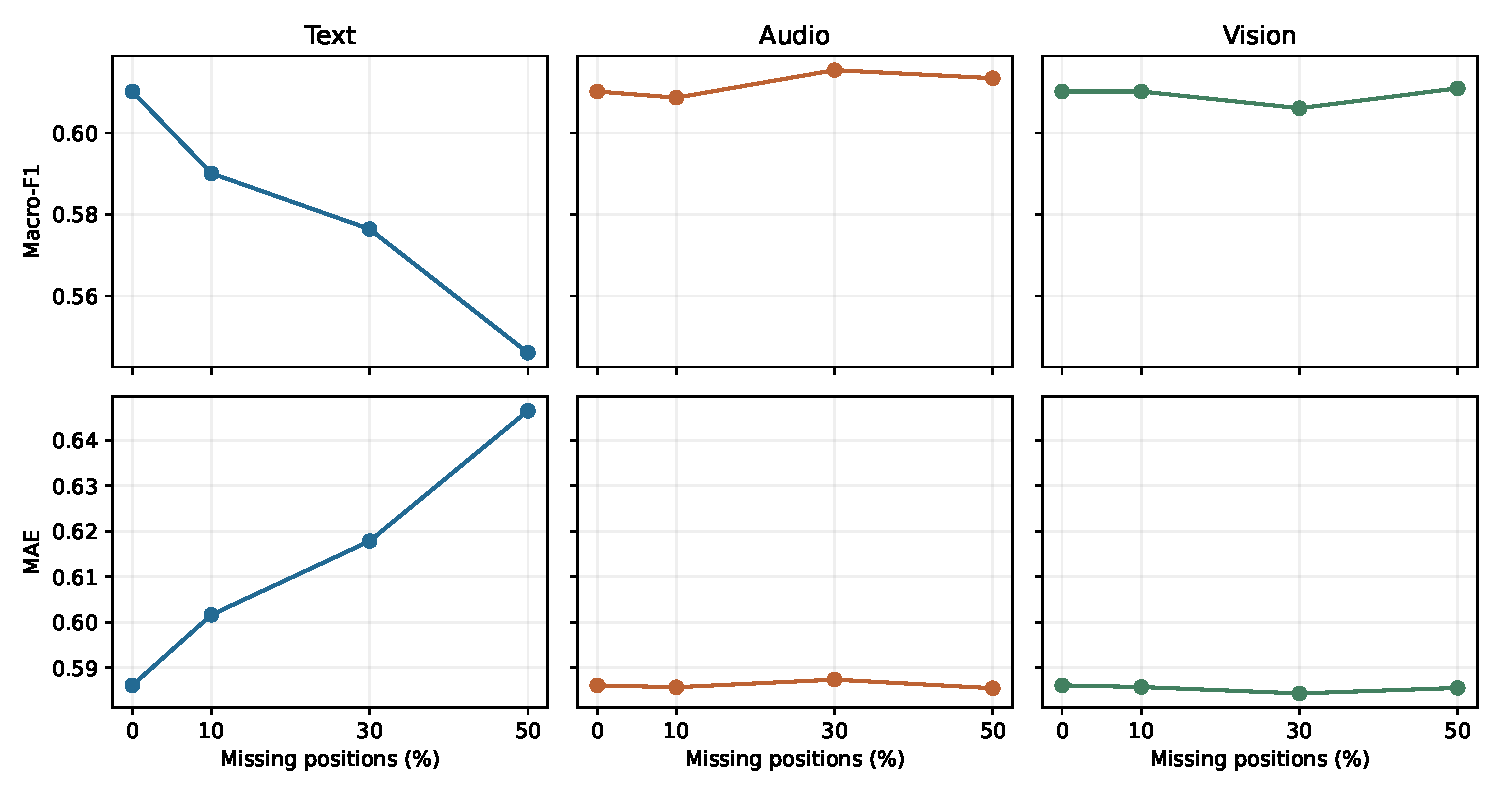
\includegraphics{../问题2/docs/final/missing.pdf}
\caption{最终模型在验证集的连续缺失比例响应。0\%为完整输入；横轴表示有效特征位置中的名义缺失比例。各行共用纵轴，F1越高越好，MAE越低越好。\label{q2-fig5}}
\end{figure}

\begin{PaperTable}{6}

\begin{table}[!htbp]
\centering\caption{最终模型的九类主要缺失场景\label{q2-tab10}}
\begin{tabular}{@{}llllll@{}}
\toprule
\begin{minipage}[b]{\dimexpr 0.130000\linewidth-1.300000\tabcolsep\relax}\raggedright
模态\strut
\end{minipage} & \begin{minipage}[b]{\dimexpr 0.120000\linewidth-1.200000\tabcolsep\relax}\raggedleft
比例\strut
\end{minipage} & \begin{minipage}[b]{\dimexpr 0.210000\linewidth-2.100000\tabcolsep\relax}\raggedleft
Macro-F1\strut
\end{minipage} & \begin{minipage}[b]{\dimexpr 0.180000\linewidth-1.800000\tabcolsep\relax}\raggedleft
ΔF1\strut
\end{minipage} & \begin{minipage}[b]{\dimexpr 0.180000\linewidth-1.800000\tabcolsep\relax}\raggedleft
MAE\strut
\end{minipage} & \begin{minipage}[b]{\dimexpr 0.180000\linewidth-1.800000\tabcolsep\relax}\raggedleft
ΔMAE\strut
\end{minipage}\tabularnewline
\midrule

\begin{minipage}[t]{\dimexpr 0.130000\linewidth-1.300000\tabcolsep\relax}\raggedright
文本\strut
\end{minipage} & \begin{minipage}[t]{\dimexpr 0.120000\linewidth-1.200000\tabcolsep\relax}\raggedleft
10\%\strut
\end{minipage} & \begin{minipage}[t]{\dimexpr 0.210000\linewidth-2.100000\tabcolsep\relax}\raggedleft
0.5901\strut
\end{minipage} & \begin{minipage}[t]{\dimexpr 0.180000\linewidth-1.800000\tabcolsep\relax}\raggedleft
-0.0201\strut
\end{minipage} & \begin{minipage}[t]{\dimexpr 0.180000\linewidth-1.800000\tabcolsep\relax}\raggedleft
0.6016\strut
\end{minipage} & \begin{minipage}[t]{\dimexpr 0.180000\linewidth-1.800000\tabcolsep\relax}\raggedleft
+0.0155\strut
\end{minipage}\tabularnewline
\begin{minipage}[t]{\dimexpr 0.130000\linewidth-1.300000\tabcolsep\relax}\raggedright
文本\strut
\end{minipage} & \begin{minipage}[t]{\dimexpr 0.120000\linewidth-1.200000\tabcolsep\relax}\raggedleft
30\%\strut
\end{minipage} & \begin{minipage}[t]{\dimexpr 0.210000\linewidth-2.100000\tabcolsep\relax}\raggedleft
0.5764\strut
\end{minipage} & \begin{minipage}[t]{\dimexpr 0.180000\linewidth-1.800000\tabcolsep\relax}\raggedleft
-0.0338\strut
\end{minipage} & \begin{minipage}[t]{\dimexpr 0.180000\linewidth-1.800000\tabcolsep\relax}\raggedleft
0.6178\strut
\end{minipage} & \begin{minipage}[t]{\dimexpr 0.180000\linewidth-1.800000\tabcolsep\relax}\raggedleft
+0.0317\strut
\end{minipage}\tabularnewline
\begin{minipage}[t]{\dimexpr 0.130000\linewidth-1.300000\tabcolsep\relax}\raggedright
文本\strut
\end{minipage} & \begin{minipage}[t]{\dimexpr 0.120000\linewidth-1.200000\tabcolsep\relax}\raggedleft
50\%\strut
\end{minipage} & \begin{minipage}[t]{\dimexpr 0.210000\linewidth-2.100000\tabcolsep\relax}\raggedleft
0.5460\strut
\end{minipage} & \begin{minipage}[t]{\dimexpr 0.180000\linewidth-1.800000\tabcolsep\relax}\raggedleft
-0.0642\strut
\end{minipage} & \begin{minipage}[t]{\dimexpr 0.180000\linewidth-1.800000\tabcolsep\relax}\raggedleft
0.6465\strut
\end{minipage} & \begin{minipage}[t]{\dimexpr 0.180000\linewidth-1.800000\tabcolsep\relax}\raggedleft
+0.0603\strut
\end{minipage}\tabularnewline
\begin{minipage}[t]{\dimexpr 0.130000\linewidth-1.300000\tabcolsep\relax}\raggedright
语音\strut
\end{minipage} & \begin{minipage}[t]{\dimexpr 0.120000\linewidth-1.200000\tabcolsep\relax}\raggedleft
10\%\strut
\end{minipage} & \begin{minipage}[t]{\dimexpr 0.210000\linewidth-2.100000\tabcolsep\relax}\raggedleft
0.6087\strut
\end{minipage} & \begin{minipage}[t]{\dimexpr 0.180000\linewidth-1.800000\tabcolsep\relax}\raggedleft
-0.0015\strut
\end{minipage} & \begin{minipage}[t]{\dimexpr 0.180000\linewidth-1.800000\tabcolsep\relax}\raggedleft
0.5857\strut
\end{minipage} & \begin{minipage}[t]{\dimexpr 0.180000\linewidth-1.800000\tabcolsep\relax}\raggedleft
-0.0004\strut
\end{minipage}\tabularnewline
\begin{minipage}[t]{\dimexpr 0.130000\linewidth-1.300000\tabcolsep\relax}\raggedright
语音\strut
\end{minipage} & \begin{minipage}[t]{\dimexpr 0.120000\linewidth-1.200000\tabcolsep\relax}\raggedleft
30\%\strut
\end{minipage} & \begin{minipage}[t]{\dimexpr 0.210000\linewidth-2.100000\tabcolsep\relax}\raggedleft
0.6154\strut
\end{minipage} & \begin{minipage}[t]{\dimexpr 0.180000\linewidth-1.800000\tabcolsep\relax}\raggedleft
+0.0052\strut
\end{minipage} & \begin{minipage}[t]{\dimexpr 0.180000\linewidth-1.800000\tabcolsep\relax}\raggedleft
0.5874\strut
\end{minipage} & \begin{minipage}[t]{\dimexpr 0.180000\linewidth-1.800000\tabcolsep\relax}\raggedleft
+0.0013\strut
\end{minipage}\tabularnewline
\begin{minipage}[t]{\dimexpr 0.130000\linewidth-1.300000\tabcolsep\relax}\raggedright
语音\strut
\end{minipage} & \begin{minipage}[t]{\dimexpr 0.120000\linewidth-1.200000\tabcolsep\relax}\raggedleft
50\%\strut
\end{minipage} & \begin{minipage}[t]{\dimexpr 0.210000\linewidth-2.100000\tabcolsep\relax}\raggedleft
0.6135\strut
\end{minipage} & \begin{minipage}[t]{\dimexpr 0.180000\linewidth-1.800000\tabcolsep\relax}\raggedleft
+0.0033\strut
\end{minipage} & \begin{minipage}[t]{\dimexpr 0.180000\linewidth-1.800000\tabcolsep\relax}\raggedleft
0.5855\strut
\end{minipage} & \begin{minipage}[t]{\dimexpr 0.180000\linewidth-1.800000\tabcolsep\relax}\raggedleft
-0.0006\strut
\end{minipage}\tabularnewline
\begin{minipage}[t]{\dimexpr 0.130000\linewidth-1.300000\tabcolsep\relax}\raggedright
视觉\strut
\end{minipage} & \begin{minipage}[t]{\dimexpr 0.120000\linewidth-1.200000\tabcolsep\relax}\raggedleft
10\%\strut
\end{minipage} & \begin{minipage}[t]{\dimexpr 0.210000\linewidth-2.100000\tabcolsep\relax}\raggedleft
0.6102\strut
\end{minipage} & \begin{minipage}[t]{\dimexpr 0.180000\linewidth-1.800000\tabcolsep\relax}\raggedleft
+0.0000\strut
\end{minipage} & \begin{minipage}[t]{\dimexpr 0.180000\linewidth-1.800000\tabcolsep\relax}\raggedleft
0.5858\strut
\end{minipage} & \begin{minipage}[t]{\dimexpr 0.180000\linewidth-1.800000\tabcolsep\relax}\raggedleft
-0.0004\strut
\end{minipage}\tabularnewline
\begin{minipage}[t]{\dimexpr 0.130000\linewidth-1.300000\tabcolsep\relax}\raggedright
视觉\strut
\end{minipage} & \begin{minipage}[t]{\dimexpr 0.120000\linewidth-1.200000\tabcolsep\relax}\raggedleft
30\%\strut
\end{minipage} & \begin{minipage}[t]{\dimexpr 0.210000\linewidth-2.100000\tabcolsep\relax}\raggedleft
0.6061\strut
\end{minipage} & \begin{minipage}[t]{\dimexpr 0.180000\linewidth-1.800000\tabcolsep\relax}\raggedleft
-0.0041\strut
\end{minipage} & \begin{minipage}[t]{\dimexpr 0.180000\linewidth-1.800000\tabcolsep\relax}\raggedleft
0.5844\strut
\end{minipage} & \begin{minipage}[t]{\dimexpr 0.180000\linewidth-1.800000\tabcolsep\relax}\raggedleft
-0.0018\strut
\end{minipage}\tabularnewline
\begin{minipage}[t]{\dimexpr 0.130000\linewidth-1.300000\tabcolsep\relax}\raggedright
视觉\strut
\end{minipage} & \begin{minipage}[t]{\dimexpr 0.120000\linewidth-1.200000\tabcolsep\relax}\raggedleft
50\%\strut
\end{minipage} & \begin{minipage}[t]{\dimexpr 0.210000\linewidth-2.100000\tabcolsep\relax}\raggedleft
0.6110\strut
\end{minipage} & \begin{minipage}[t]{\dimexpr 0.180000\linewidth-1.800000\tabcolsep\relax}\raggedleft
+0.0008\strut
\end{minipage} & \begin{minipage}[t]{\dimexpr 0.180000\linewidth-1.800000\tabcolsep\relax}\raggedleft
0.5856\strut
\end{minipage} & \begin{minipage}[t]{\dimexpr 0.180000\linewidth-1.800000\tabcolsep\relax}\raggedleft
-0.0006\strut
\end{minipage}\tabularnewline
\bottomrule
\end{tabular}
\end{table}

\end{PaperTable}

九类场景平均Macro-F1为0.5975，平均MAE为0.5978。文本连续缺失50\%时，F1相对完整输入变化-0.0642，MAE变化+0.0603。音视频缺失的影响较小且存在非单调变化；这与当前模型对文本的依赖及音视频均值表示相容，但不足以单独证明噪声移除或模态冗余等机制。

\hypertarget{q2-ux7f3aux5931ux4f4dux7f6eux4e0eux7247ux6bb5ux957fux5ea6}{%
\paragraph{缺失位置与片段长度}\label{q2-ux7f3aux5931ux4f4dux7f6eux4e0eux7247ux6bb5ux957fux5ea6}}

附件2提供对齐序列位置而非逐词时间戳，缺失长度按有效位置数及比例定义。前部、中部、后部采用相同移除数量，不将位置比例换算为秒数。随机连续区间之外，另评价多个短段，共36类补充场景。

固定文本缺失比例50\%时，前部、中部、后部的Macro-F1分别为0.5716、0.5381、0.5043。这一差异说明相同缺失比例下，删除位置仍会影响预测。该结果描述当前样本与模型，不能直接归因为某个时间段承载更多情绪。

\begin{PaperTable}{3}

\begin{table}[!htbp]
\centering\caption{文本多短段缺失相对单连续区间的差值\label{q2-tab19}}
\begin{tabular}{@{}lll@{}}
\toprule
\begin{minipage}[b]{\dimexpr 0.280000\linewidth-1.120000\tabcolsep\relax}\raggedleft
缺失比例\strut
\end{minipage} & \begin{minipage}[b]{\dimexpr 0.360000\linewidth-1.440000\tabcolsep\relax}\raggedleft
ΔMacro-F1\strut
\end{minipage} & \begin{minipage}[b]{\dimexpr 0.360000\linewidth-1.440000\tabcolsep\relax}\raggedleft
ΔMAE\strut
\end{minipage}\tabularnewline
\midrule

\begin{minipage}[t]{\dimexpr 0.280000\linewidth-1.120000\tabcolsep\relax}\raggedleft
10\%\strut
\end{minipage} & \begin{minipage}[t]{\dimexpr 0.360000\linewidth-1.440000\tabcolsep\relax}\raggedleft
+0.0028\strut
\end{minipage} & \begin{minipage}[t]{\dimexpr 0.360000\linewidth-1.440000\tabcolsep\relax}\raggedleft
-0.0036\strut
\end{minipage}\tabularnewline
\begin{minipage}[t]{\dimexpr 0.280000\linewidth-1.120000\tabcolsep\relax}\raggedleft
30\%\strut
\end{minipage} & \begin{minipage}[t]{\dimexpr 0.360000\linewidth-1.440000\tabcolsep\relax}\raggedleft
-0.0033\strut
\end{minipage} & \begin{minipage}[t]{\dimexpr 0.360000\linewidth-1.440000\tabcolsep\relax}\raggedleft
+0.0061\strut
\end{minipage}\tabularnewline
\begin{minipage}[t]{\dimexpr 0.280000\linewidth-1.120000\tabcolsep\relax}\raggedleft
50\%\strut
\end{minipage} & \begin{minipage}[t]{\dimexpr 0.360000\linewidth-1.440000\tabcolsep\relax}\raggedleft
-0.0164\strut
\end{minipage} & \begin{minipage}[t]{\dimexpr 0.360000\linewidth-1.440000\tabcolsep\relax}\raggedleft
-0.0060\strut
\end{minipage}\tabularnewline
\bottomrule
\end{tabular}
\end{table}

\end{PaperTable}

多短段与单长段的变化按分类、回归分别判断；极短序列中的相邻短段可能合并。名义比例10\%、30\%、50\%对应样本平均实际位置比例11.20\%、30.74\%、51.64\%，偏差来自取整及至少移除一个位置。若原位置已不可观测，新增信息损失小于所选位置数。

\begin{figure}
\centering
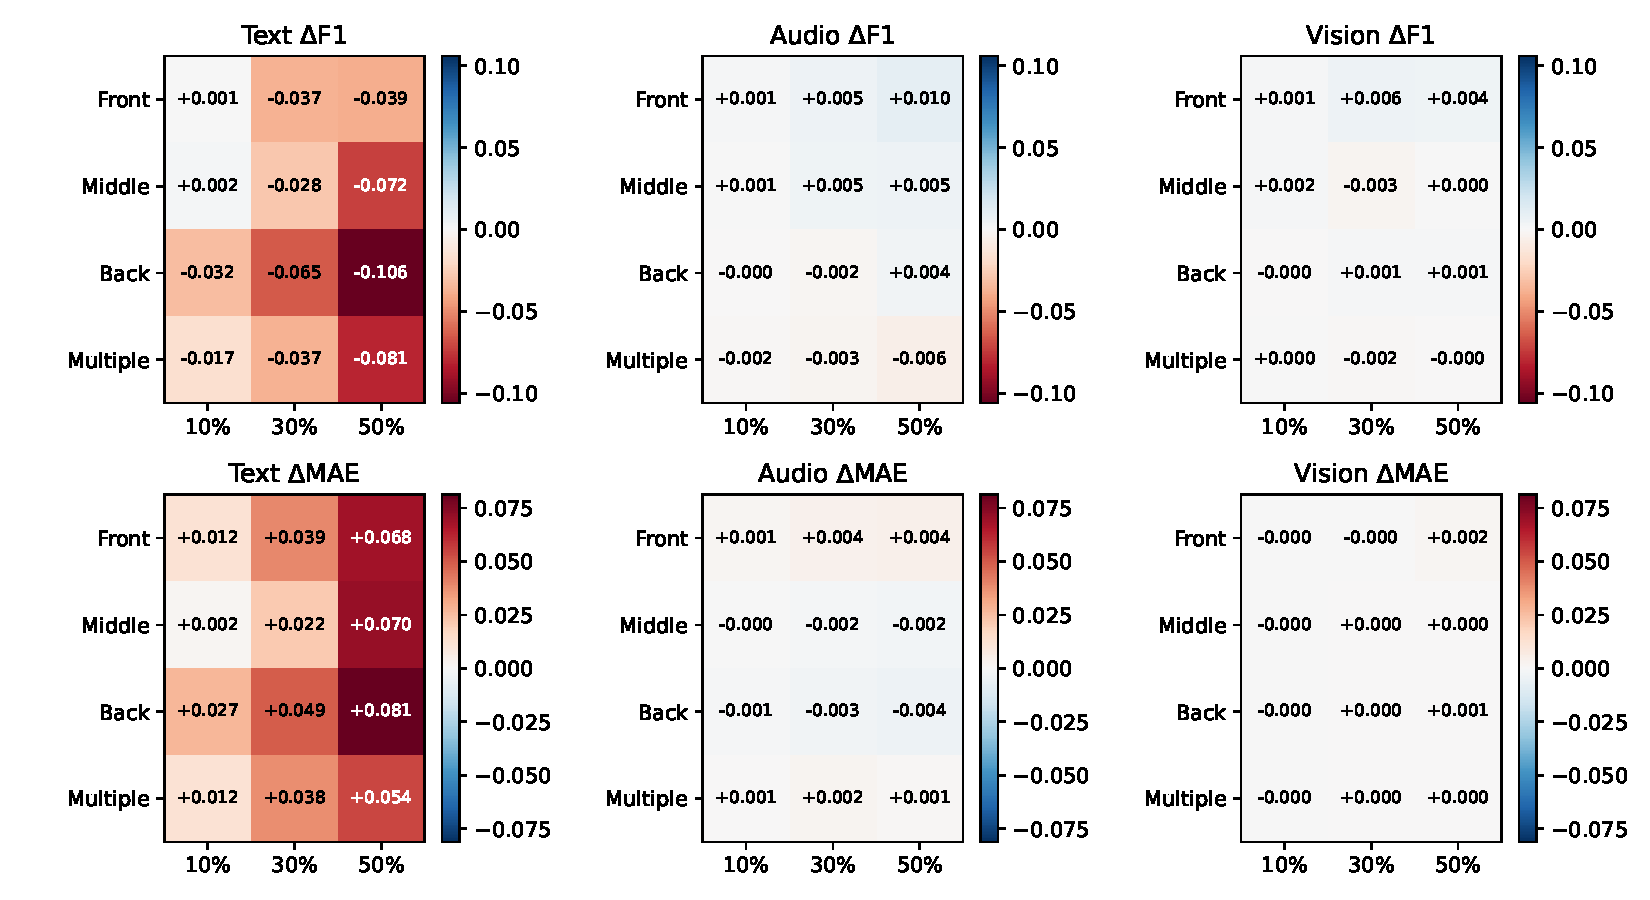
\includegraphics{../问题2/docs/final/missing_shapes.pdf}
\caption{最终模型的36类位置与形状对照。上排为相对完整输入的F1变化，下排为MAE变化；同一指标共用色标。\label{q2-fig6}}
\end{figure}

\hypertarget{q2-ux5206ux7c7bux4e0eux56deux5f52ux8befux5dee}{%
\subsubsection{分类与回归误差}\label{q2-ux5206ux7c7bux4e0eux56deux5f52ux8befux5dee}}

\begin{figure}
\centering
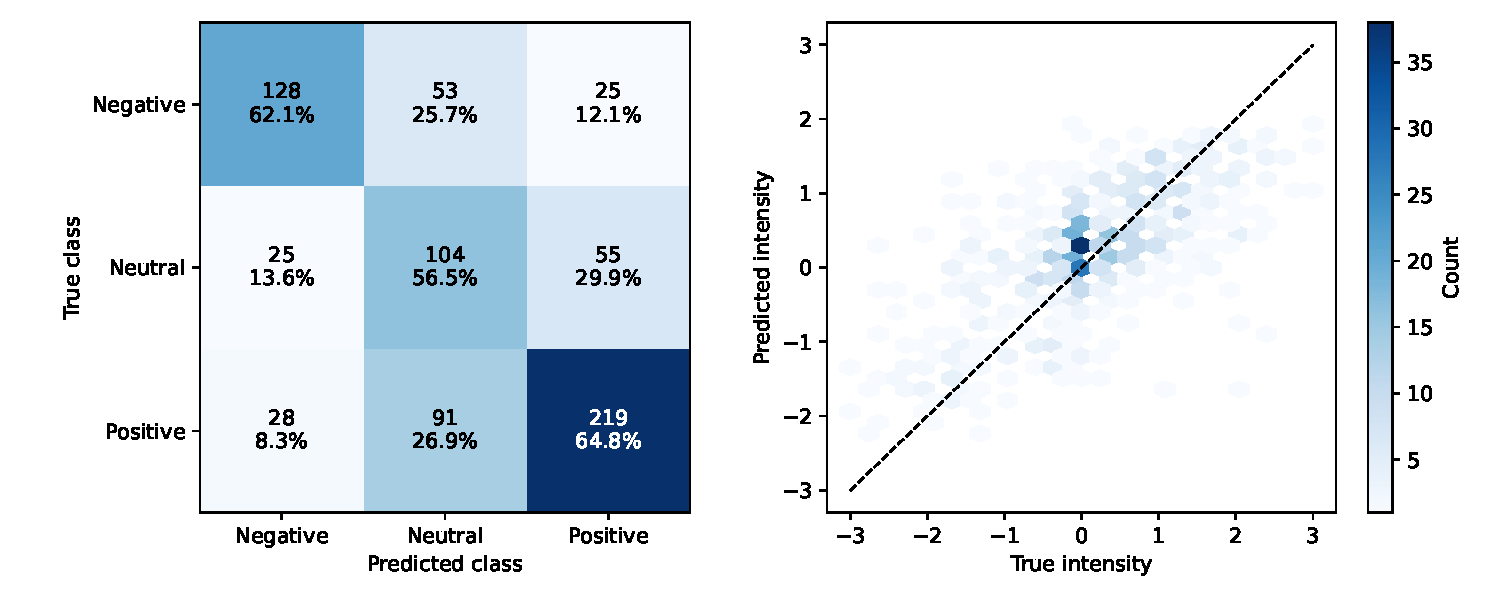
\includegraphics{../问题2/docs/final/errors.pdf}
\caption{最终模型在728条验证样本上的错误分析。左图为混淆矩阵，格内显示计数及真实类别内比例；右图为真实强度与预测强度的二维计数，虚线表示理想预测。\label{q2-fig7}}
\end{figure}

负向、中性、正向的F1分别为0.6615、0.4815、0.6876。184条中性样本中，104条识别正确，25条误判为负向，55条误判为正向；中性与有倾向情感之间的混淆是主要分类难点。

三个真实类别的MAE分别为0.7981、0.4116、0.5519，负向样本的强度误差较大。混淆矩阵与强度散点提供错误分布证据；具体语言歧义或情境缺失是否造成错误，仍须逐样本证据支持。

分类与回归由两个任务头分别监督。完整验证集有248条样本预测为中性但回归值不为精确零，另有14条非中性分类与回归正负方向相反。前者可能包含接近零的连续输出，两类情况分开报告；评价分别使用离散真值和连续真值，不根据这些结果另行调整中性阈值。

\hypertarget{q2-ux9644ux4ef6ux4e09ux5168ux91cfux9884ux6d4bux4e0eux7ed3ux679cux63a5ux53e3}{%
\subsection{附件三全量预测与结果接口}\label{q2-ux9644ux4ef6ux4e09ux5168ux91cfux9884ux6d4bux4e0eux7ed3ux679cux63a5ux53e3}}

30条样本采用最终重训模型、同一对齐版本与训练集标准化统计。按文件名及文件内序号构造样本标识，检查整数词元编号、形状、有限性与观测掩码后，输出三类概率、极性和强度。

\begin{PaperTable}{4}

\begin{longtable}[]{@{}llll@{}}
\caption{附件3全部30条类别平衡模型预测\label{q2-tab17}}\tabularnewline
\toprule
\begin{minipage}[b]{\dimexpr 0.300000\linewidth-1.800000\tabcolsep\relax}\raggedright
文件编号\strut
\end{minipage} & \begin{minipage}[b]{\dimexpr 0.200000\linewidth-1.200000\tabcolsep\relax}\raggedright
预测类别\strut
\end{minipage} & \begin{minipage}[b]{\dimexpr 0.250000\linewidth-1.500000\tabcolsep\relax}\raggedleft
情感强度\strut
\end{minipage} & \begin{minipage}[b]{\dimexpr 0.250000\linewidth-1.500000\tabcolsep\relax}\raggedleft
最大类概率\strut
\end{minipage}\tabularnewline
\midrule
\endfirsthead
\caption[]{附件3全部30条类别平衡模型预测（续）}\tabularnewline
\toprule
\begin{minipage}[b]{\dimexpr 0.300000\linewidth-1.800000\tabcolsep\relax}\raggedright
文件编号\strut
\end{minipage} & \begin{minipage}[b]{\dimexpr 0.200000\linewidth-1.200000\tabcolsep\relax}\raggedright
预测类别\strut
\end{minipage} & \begin{minipage}[b]{\dimexpr 0.250000\linewidth-1.500000\tabcolsep\relax}\raggedleft
情感强度\strut
\end{minipage} & \begin{minipage}[b]{\dimexpr 0.250000\linewidth-1.500000\tabcolsep\relax}\raggedleft
最大类概率\strut
\end{minipage}\tabularnewline
\midrule
\endhead
\begin{minipage}[t]{\dimexpr 0.300000\linewidth-1.800000\tabcolsep\relax}\raggedright
附件3\_01\strut
\end{minipage} & \begin{minipage}[t]{\dimexpr 0.200000\linewidth-1.200000\tabcolsep\relax}\raggedright
负向\strut
\end{minipage} & \begin{minipage}[t]{\dimexpr 0.250000\linewidth-1.500000\tabcolsep\relax}\raggedleft
-0.7402\strut
\end{minipage} & \begin{minipage}[t]{\dimexpr 0.250000\linewidth-1.500000\tabcolsep\relax}\raggedleft
0.8852\strut
\end{minipage}\tabularnewline
\begin{minipage}[t]{\dimexpr 0.300000\linewidth-1.800000\tabcolsep\relax}\raggedright
附件3\_02\strut
\end{minipage} & \begin{minipage}[t]{\dimexpr 0.200000\linewidth-1.200000\tabcolsep\relax}\raggedright
中性\strut
\end{minipage} & \begin{minipage}[t]{\dimexpr 0.250000\linewidth-1.500000\tabcolsep\relax}\raggedleft
0.0432\strut
\end{minipage} & \begin{minipage}[t]{\dimexpr 0.250000\linewidth-1.500000\tabcolsep\relax}\raggedleft
0.8140\strut
\end{minipage}\tabularnewline
\begin{minipage}[t]{\dimexpr 0.300000\linewidth-1.800000\tabcolsep\relax}\raggedright
附件3\_03\strut
\end{minipage} & \begin{minipage}[t]{\dimexpr 0.200000\linewidth-1.200000\tabcolsep\relax}\raggedright
中性\strut
\end{minipage} & \begin{minipage}[t]{\dimexpr 0.250000\linewidth-1.500000\tabcolsep\relax}\raggedleft
0.3155\strut
\end{minipage} & \begin{minipage}[t]{\dimexpr 0.250000\linewidth-1.500000\tabcolsep\relax}\raggedleft
0.6738\strut
\end{minipage}\tabularnewline
\begin{minipage}[t]{\dimexpr 0.300000\linewidth-1.800000\tabcolsep\relax}\raggedright
附件3\_04\strut
\end{minipage} & \begin{minipage}[t]{\dimexpr 0.200000\linewidth-1.200000\tabcolsep\relax}\raggedright
正向\strut
\end{minipage} & \begin{minipage}[t]{\dimexpr 0.250000\linewidth-1.500000\tabcolsep\relax}\raggedleft
0.4635\strut
\end{minipage} & \begin{minipage}[t]{\dimexpr 0.250000\linewidth-1.500000\tabcolsep\relax}\raggedleft
0.5250\strut
\end{minipage}\tabularnewline
\begin{minipage}[t]{\dimexpr 0.300000\linewidth-1.800000\tabcolsep\relax}\raggedright
附件3\_05\strut
\end{minipage} & \begin{minipage}[t]{\dimexpr 0.200000\linewidth-1.200000\tabcolsep\relax}\raggedright
负向\strut
\end{minipage} & \begin{minipage}[t]{\dimexpr 0.250000\linewidth-1.500000\tabcolsep\relax}\raggedleft
-1.2858\strut
\end{minipage} & \begin{minipage}[t]{\dimexpr 0.250000\linewidth-1.500000\tabcolsep\relax}\raggedleft
0.9375\strut
\end{minipage}\tabularnewline
\begin{minipage}[t]{\dimexpr 0.300000\linewidth-1.800000\tabcolsep\relax}\raggedright
附件3\_06\strut
\end{minipage} & \begin{minipage}[t]{\dimexpr 0.200000\linewidth-1.200000\tabcolsep\relax}\raggedright
正向\strut
\end{minipage} & \begin{minipage}[t]{\dimexpr 0.250000\linewidth-1.500000\tabcolsep\relax}\raggedleft
0.7481\strut
\end{minipage} & \begin{minipage}[t]{\dimexpr 0.250000\linewidth-1.500000\tabcolsep\relax}\raggedleft
0.7617\strut
\end{minipage}\tabularnewline
\begin{minipage}[t]{\dimexpr 0.300000\linewidth-1.800000\tabcolsep\relax}\raggedright
附件3\_07\strut
\end{minipage} & \begin{minipage}[t]{\dimexpr 0.200000\linewidth-1.200000\tabcolsep\relax}\raggedright
正向\strut
\end{minipage} & \begin{minipage}[t]{\dimexpr 0.250000\linewidth-1.500000\tabcolsep\relax}\raggedleft
0.3521\strut
\end{minipage} & \begin{minipage}[t]{\dimexpr 0.250000\linewidth-1.500000\tabcolsep\relax}\raggedleft
0.4673\strut
\end{minipage}\tabularnewline
\begin{minipage}[t]{\dimexpr 0.300000\linewidth-1.800000\tabcolsep\relax}\raggedright
附件3\_08\strut
\end{minipage} & \begin{minipage}[t]{\dimexpr 0.200000\linewidth-1.200000\tabcolsep\relax}\raggedright
中性\strut
\end{minipage} & \begin{minipage}[t]{\dimexpr 0.250000\linewidth-1.500000\tabcolsep\relax}\raggedleft
0.1078\strut
\end{minipage} & \begin{minipage}[t]{\dimexpr 0.250000\linewidth-1.500000\tabcolsep\relax}\raggedleft
0.5762\strut
\end{minipage}\tabularnewline
\begin{minipage}[t]{\dimexpr 0.300000\linewidth-1.800000\tabcolsep\relax}\raggedright
附件3\_09\strut
\end{minipage} & \begin{minipage}[t]{\dimexpr 0.200000\linewidth-1.200000\tabcolsep\relax}\raggedright
正向\strut
\end{minipage} & \begin{minipage}[t]{\dimexpr 0.250000\linewidth-1.500000\tabcolsep\relax}\raggedleft
1.3437\strut
\end{minipage} & \begin{minipage}[t]{\dimexpr 0.250000\linewidth-1.500000\tabcolsep\relax}\raggedleft
0.9423\strut
\end{minipage}\tabularnewline
\begin{minipage}[t]{\dimexpr 0.300000\linewidth-1.800000\tabcolsep\relax}\raggedright
附件3\_10\strut
\end{minipage} & \begin{minipage}[t]{\dimexpr 0.200000\linewidth-1.200000\tabcolsep\relax}\raggedright
中性\strut
\end{minipage} & \begin{minipage}[t]{\dimexpr 0.250000\linewidth-1.500000\tabcolsep\relax}\raggedleft
-0.0757\strut
\end{minipage} & \begin{minipage}[t]{\dimexpr 0.250000\linewidth-1.500000\tabcolsep\relax}\raggedleft
0.8782\strut
\end{minipage}\tabularnewline
\begin{minipage}[t]{\dimexpr 0.300000\linewidth-1.800000\tabcolsep\relax}\raggedright
附件3\_11\strut
\end{minipage} & \begin{minipage}[t]{\dimexpr 0.200000\linewidth-1.200000\tabcolsep\relax}\raggedright
正向\strut
\end{minipage} & \begin{minipage}[t]{\dimexpr 0.250000\linewidth-1.500000\tabcolsep\relax}\raggedleft
0.4526\strut
\end{minipage} & \begin{minipage}[t]{\dimexpr 0.250000\linewidth-1.500000\tabcolsep\relax}\raggedleft
0.5042\strut
\end{minipage}\tabularnewline
\begin{minipage}[t]{\dimexpr 0.300000\linewidth-1.800000\tabcolsep\relax}\raggedright
附件3\_12\strut
\end{minipage} & \begin{minipage}[t]{\dimexpr 0.200000\linewidth-1.200000\tabcolsep\relax}\raggedright
正向\strut
\end{minipage} & \begin{minipage}[t]{\dimexpr 0.250000\linewidth-1.500000\tabcolsep\relax}\raggedleft
0.5467\strut
\end{minipage} & \begin{minipage}[t]{\dimexpr 0.250000\linewidth-1.500000\tabcolsep\relax}\raggedleft
0.5337\strut
\end{minipage}\tabularnewline
\begin{minipage}[t]{\dimexpr 0.300000\linewidth-1.800000\tabcolsep\relax}\raggedright
附件3\_13\strut
\end{minipage} & \begin{minipage}[t]{\dimexpr 0.200000\linewidth-1.200000\tabcolsep\relax}\raggedright
正向\strut
\end{minipage} & \begin{minipage}[t]{\dimexpr 0.250000\linewidth-1.500000\tabcolsep\relax}\raggedleft
0.3173\strut
\end{minipage} & \begin{minipage}[t]{\dimexpr 0.250000\linewidth-1.500000\tabcolsep\relax}\raggedleft
0.5285\strut
\end{minipage}\tabularnewline
\begin{minipage}[t]{\dimexpr 0.300000\linewidth-1.800000\tabcolsep\relax}\raggedright
附件3\_14\strut
\end{minipage} & \begin{minipage}[t]{\dimexpr 0.200000\linewidth-1.200000\tabcolsep\relax}\raggedright
负向\strut
\end{minipage} & \begin{minipage}[t]{\dimexpr 0.250000\linewidth-1.500000\tabcolsep\relax}\raggedleft
-0.7928\strut
\end{minipage} & \begin{minipage}[t]{\dimexpr 0.250000\linewidth-1.500000\tabcolsep\relax}\raggedleft
0.9172\strut
\end{minipage}\tabularnewline
\begin{minipage}[t]{\dimexpr 0.300000\linewidth-1.800000\tabcolsep\relax}\raggedright
附件3\_15\strut
\end{minipage} & \begin{minipage}[t]{\dimexpr 0.200000\linewidth-1.200000\tabcolsep\relax}\raggedright
正向\strut
\end{minipage} & \begin{minipage}[t]{\dimexpr 0.250000\linewidth-1.500000\tabcolsep\relax}\raggedleft
0.5340\strut
\end{minipage} & \begin{minipage}[t]{\dimexpr 0.250000\linewidth-1.500000\tabcolsep\relax}\raggedleft
0.7418\strut
\end{minipage}\tabularnewline
\begin{minipage}[t]{\dimexpr 0.300000\linewidth-1.800000\tabcolsep\relax}\raggedright
附件3\_16\strut
\end{minipage} & \begin{minipage}[t]{\dimexpr 0.200000\linewidth-1.200000\tabcolsep\relax}\raggedright
正向\strut
\end{minipage} & \begin{minipage}[t]{\dimexpr 0.250000\linewidth-1.500000\tabcolsep\relax}\raggedleft
1.5088\strut
\end{minipage} & \begin{minipage}[t]{\dimexpr 0.250000\linewidth-1.500000\tabcolsep\relax}\raggedleft
0.9448\strut
\end{minipage}\tabularnewline
\begin{minipage}[t]{\dimexpr 0.300000\linewidth-1.800000\tabcolsep\relax}\raggedright
附件3\_17\strut
\end{minipage} & \begin{minipage}[t]{\dimexpr 0.200000\linewidth-1.200000\tabcolsep\relax}\raggedright
中性\strut
\end{minipage} & \begin{minipage}[t]{\dimexpr 0.250000\linewidth-1.500000\tabcolsep\relax}\raggedleft
0.1920\strut
\end{minipage} & \begin{minipage}[t]{\dimexpr 0.250000\linewidth-1.500000\tabcolsep\relax}\raggedleft
0.6818\strut
\end{minipage}\tabularnewline
\begin{minipage}[t]{\dimexpr 0.300000\linewidth-1.800000\tabcolsep\relax}\raggedright
附件3\_18\strut
\end{minipage} & \begin{minipage}[t]{\dimexpr 0.200000\linewidth-1.200000\tabcolsep\relax}\raggedright
正向\strut
\end{minipage} & \begin{minipage}[t]{\dimexpr 0.250000\linewidth-1.500000\tabcolsep\relax}\raggedleft
0.4755\strut
\end{minipage} & \begin{minipage}[t]{\dimexpr 0.250000\linewidth-1.500000\tabcolsep\relax}\raggedleft
0.5403\strut
\end{minipage}\tabularnewline
\begin{minipage}[t]{\dimexpr 0.300000\linewidth-1.800000\tabcolsep\relax}\raggedright
附件3\_19\strut
\end{minipage} & \begin{minipage}[t]{\dimexpr 0.200000\linewidth-1.200000\tabcolsep\relax}\raggedright
中性\strut
\end{minipage} & \begin{minipage}[t]{\dimexpr 0.250000\linewidth-1.500000\tabcolsep\relax}\raggedleft
-0.1132\strut
\end{minipage} & \begin{minipage}[t]{\dimexpr 0.250000\linewidth-1.500000\tabcolsep\relax}\raggedleft
0.4775\strut
\end{minipage}\tabularnewline
\begin{minipage}[t]{\dimexpr 0.300000\linewidth-1.800000\tabcolsep\relax}\raggedright
附件3\_20\strut
\end{minipage} & \begin{minipage}[t]{\dimexpr 0.200000\linewidth-1.200000\tabcolsep\relax}\raggedright
中性\strut
\end{minipage} & \begin{minipage}[t]{\dimexpr 0.250000\linewidth-1.500000\tabcolsep\relax}\raggedleft
0.1702\strut
\end{minipage} & \begin{minipage}[t]{\dimexpr 0.250000\linewidth-1.500000\tabcolsep\relax}\raggedleft
0.7382\strut
\end{minipage}\tabularnewline
\begin{minipage}[t]{\dimexpr 0.300000\linewidth-1.800000\tabcolsep\relax}\raggedright
附件3\_21\strut
\end{minipage} & \begin{minipage}[t]{\dimexpr 0.200000\linewidth-1.200000\tabcolsep\relax}\raggedright
正向\strut
\end{minipage} & \begin{minipage}[t]{\dimexpr 0.250000\linewidth-1.500000\tabcolsep\relax}\raggedleft
0.4119\strut
\end{minipage} & \begin{minipage}[t]{\dimexpr 0.250000\linewidth-1.500000\tabcolsep\relax}\raggedleft
0.5905\strut
\end{minipage}\tabularnewline
\begin{minipage}[t]{\dimexpr 0.300000\linewidth-1.800000\tabcolsep\relax}\raggedright
附件3\_22\strut
\end{minipage} & \begin{minipage}[t]{\dimexpr 0.200000\linewidth-1.200000\tabcolsep\relax}\raggedright
正向\strut
\end{minipage} & \begin{minipage}[t]{\dimexpr 0.250000\linewidth-1.500000\tabcolsep\relax}\raggedleft
0.5062\strut
\end{minipage} & \begin{minipage}[t]{\dimexpr 0.250000\linewidth-1.500000\tabcolsep\relax}\raggedleft
0.5876\strut
\end{minipage}\tabularnewline
\begin{minipage}[t]{\dimexpr 0.300000\linewidth-1.800000\tabcolsep\relax}\raggedright
附件3\_23\strut
\end{minipage} & \begin{minipage}[t]{\dimexpr 0.200000\linewidth-1.200000\tabcolsep\relax}\raggedright
中性\strut
\end{minipage} & \begin{minipage}[t]{\dimexpr 0.250000\linewidth-1.500000\tabcolsep\relax}\raggedleft
0.4318\strut
\end{minipage} & \begin{minipage}[t]{\dimexpr 0.250000\linewidth-1.500000\tabcolsep\relax}\raggedleft
0.4883\strut
\end{minipage}\tabularnewline
\begin{minipage}[t]{\dimexpr 0.300000\linewidth-1.800000\tabcolsep\relax}\raggedright
附件3\_24\strut
\end{minipage} & \begin{minipage}[t]{\dimexpr 0.200000\linewidth-1.200000\tabcolsep\relax}\raggedright
中性\strut
\end{minipage} & \begin{minipage}[t]{\dimexpr 0.250000\linewidth-1.500000\tabcolsep\relax}\raggedleft
0.0165\strut
\end{minipage} & \begin{minipage}[t]{\dimexpr 0.250000\linewidth-1.500000\tabcolsep\relax}\raggedleft
0.3973\strut
\end{minipage}\tabularnewline
\begin{minipage}[t]{\dimexpr 0.300000\linewidth-1.800000\tabcolsep\relax}\raggedright
附件3\_25\strut
\end{minipage} & \begin{minipage}[t]{\dimexpr 0.200000\linewidth-1.200000\tabcolsep\relax}\raggedright
中性\strut
\end{minipage} & \begin{minipage}[t]{\dimexpr 0.250000\linewidth-1.500000\tabcolsep\relax}\raggedleft
0.3023\strut
\end{minipage} & \begin{minipage}[t]{\dimexpr 0.250000\linewidth-1.500000\tabcolsep\relax}\raggedleft
0.7077\strut
\end{minipage}\tabularnewline
\begin{minipage}[t]{\dimexpr 0.300000\linewidth-1.800000\tabcolsep\relax}\raggedright
附件3\_26\strut
\end{minipage} & \begin{minipage}[t]{\dimexpr 0.200000\linewidth-1.200000\tabcolsep\relax}\raggedright
正向\strut
\end{minipage} & \begin{minipage}[t]{\dimexpr 0.250000\linewidth-1.500000\tabcolsep\relax}\raggedleft
0.6231\strut
\end{minipage} & \begin{minipage}[t]{\dimexpr 0.250000\linewidth-1.500000\tabcolsep\relax}\raggedleft
0.7085\strut
\end{minipage}\tabularnewline
\begin{minipage}[t]{\dimexpr 0.300000\linewidth-1.800000\tabcolsep\relax}\raggedright
附件3\_27\strut
\end{minipage} & \begin{minipage}[t]{\dimexpr 0.200000\linewidth-1.200000\tabcolsep\relax}\raggedright
正向\strut
\end{minipage} & \begin{minipage}[t]{\dimexpr 0.250000\linewidth-1.500000\tabcolsep\relax}\raggedleft
0.4430\strut
\end{minipage} & \begin{minipage}[t]{\dimexpr 0.250000\linewidth-1.500000\tabcolsep\relax}\raggedleft
0.6133\strut
\end{minipage}\tabularnewline
\begin{minipage}[t]{\dimexpr 0.300000\linewidth-1.800000\tabcolsep\relax}\raggedright
附件3\_28\strut
\end{minipage} & \begin{minipage}[t]{\dimexpr 0.200000\linewidth-1.200000\tabcolsep\relax}\raggedright
正向\strut
\end{minipage} & \begin{minipage}[t]{\dimexpr 0.250000\linewidth-1.500000\tabcolsep\relax}\raggedleft
0.6392\strut
\end{minipage} & \begin{minipage}[t]{\dimexpr 0.250000\linewidth-1.500000\tabcolsep\relax}\raggedleft
0.5539\strut
\end{minipage}\tabularnewline
\begin{minipage}[t]{\dimexpr 0.300000\linewidth-1.800000\tabcolsep\relax}\raggedright
附件3\_29\strut
\end{minipage} & \begin{minipage}[t]{\dimexpr 0.200000\linewidth-1.200000\tabcolsep\relax}\raggedright
正向\strut
\end{minipage} & \begin{minipage}[t]{\dimexpr 0.250000\linewidth-1.500000\tabcolsep\relax}\raggedleft
0.6799\strut
\end{minipage} & \begin{minipage}[t]{\dimexpr 0.250000\linewidth-1.500000\tabcolsep\relax}\raggedleft
0.6390\strut
\end{minipage}\tabularnewline
\begin{minipage}[t]{\dimexpr 0.300000\linewidth-1.800000\tabcolsep\relax}\raggedright
附件3\_30\strut
\end{minipage} & \begin{minipage}[t]{\dimexpr 0.200000\linewidth-1.200000\tabcolsep\relax}\raggedright
中性\strut
\end{minipage} & \begin{minipage}[t]{\dimexpr 0.250000\linewidth-1.500000\tabcolsep\relax}\raggedleft
0.4845\strut
\end{minipage} & \begin{minipage}[t]{\dimexpr 0.250000\linewidth-1.500000\tabcolsep\relax}\raggedleft
0.6779\strut
\end{minipage}\tabularnewline
\bottomrule
\end{longtable}

\end{PaperTable}

结果文件为\texttt{attachme\allowbreak{}nt3\_\allowbreak{}predicti\allowbreak{}ons.csv}，保留sample\_id、scenario、class\_id、sentiment、intensity和三类概率，表内数值为显示而舍入，CSV保留原计算精度。稳定标识使用文件名和文件内序号，与原始视频标识分开保存。附件3没有标签，其预测分布不用于调参，最大类概率也不是已校准的置信度。

文本编码的主要计算量为 \(O(L(Td^2+T^2d+Td\,d_{ff}))\)，其中T=50、d=768、L=12；音视汇总分别为 \(O(74T)\)、\(O(35T)\)。运行环境使用Python 3.10、PyTorch 2.8.0+cu128、CUDA 12.8、NumPy 2.2.6和scikit-learn 1.7.2，精确依赖版本随环境文件保存。独立复算需要与模型记录中SHA256一致的权重和标准化参数，先构造同一观测掩码，再进行批量推理。固定模型与标准化参数均已保存。CPU重放附件三30条预测时，类别与已保存结果全部一致，强度最大绝对差为\(2.15\times10^{-6}\)；单条与批量推理类别一致，重新加载模型后输出完全一致。

\hypertarget{q2-ux672cux95eeux5c0fux7ed3}{%
\subsection{本问小结}\label{q2-ux672cux95eeux5c0fux7ed3}}

最终模型在728条验证样本上的Accuracy为0.6195、Macro-F1为0.6102、MAE为0.5861、Pearson为0.6712。文本缺失的影响较大，缺失位置与片段长度也会改变分类和回归结果。固定4轮的配对消融中，关闭连续缺失增强后，50\%共同缺失的F1由0.5300降至0.5237，46个评价场景的三折平均MAE均增加；因此保留原连续缺失增强方案。该结论限定于所列训练设置、观测策略和评价场景，最终模型与历史三个随机种子的选择结果分别报告。
